%%%%%%%%%%%%%%%%%%%%%%%%%%%%%%%%%%%%%%%%%%%%%%%%%%%%%%%%%%%%%%%%%%%%%%%%%%%%%%%%
%% Plantilla de memoria en LaTeX para la ETSIT - Universidad Rey Juan Carlos
%%
%% Por Gregorio Robles <grex arroba gsyc.urjc.es>
%%     Grupo de Sistemas y Comunicaciones
%%     Escuela Técnica Superior de Ingenieros de Telecomunicación
%%     Universidad Rey Juan Carlos
%% (muchas ideas tomadas de Internet, colegas del GSyC, antiguos alumnos...
%%  etc. Muchas gracias a todos)
%%
%% La última versión de esta plantilla está siempre disponible en:
%%     https://github.com/gregoriorobles/plantilla-memoria
%%
%% Para obtener PDF, ejecuta en la shell:
%%   make
%% (las imágenes deben ir en PNG o JPG)

%%%%%%%%%%%%%%%%%%%%%%%%%%%%%%%%%%%%%%%%%%%%%%%%%%%%%%%%%%%%%%%%%%%%%%%%%%%%%%%%

\documentclass[a4paper, 12pt]{book}
%\usepackage[T1]{fontenc}

\usepackage[a4paper, left=2.5cm, right=2.5cm, top=3cm, bottom=3cm]{geometry}
\usepackage{times}
\usepackage[utf8]{inputenc}
\usepackage[spanish]{babel} % Comenta esta línea si tu memoria es en inglés
\usepackage{url}
%\usepackage[dvipdfm]{graphicx}
\usepackage{graphicx}
\usepackage{float}  %% H para posicionar figuras
\usepackage[nottoc, notlot, notlof, notindex]{tocbibind} %% Opciones de índice
\usepackage{latexsym}  %% Logo LaTeX
\usepackage{amsmath}
\usepackage{graphicx}
\usepackage{subcaption}

\title{Memoria del Proyecto}
\author{Carmen González López}

\renewcommand{\baselinestretch}{1.5}  %% Interlineado

\begin{document}

\renewcommand{\refname}{Bibliografía}  %% Renombrando
\renewcommand{\appendixname}{Apéndice}

%%%%%%%%%%%%%%%%%%%%%%%%%%%%%%%%%%%%%%%%%%%%%%%%%%%%%%%%%%%%%%%%%%%%%%%%%%%%%%%%
% PORTADA

\begin{titlepage}
\begin{center}
\includegraphics[scale=0.6]{img/URJ_logo_Color_POS.png}

\vspace{1.75cm}

\LARGE
ESCUELA DE INGENIERÍA DE FUENLABRADA
\vspace{1cm}

\LARGE
GRADO EN INGENIERÍA EN SISTEMAS AUDIOVISUALES Y MULTIMEDIA

\vspace{1cm}
\LARGE
\textbf{TRABAJO FIN DE GRADO}

\vspace{2cm}

\Large
ANÁLISIS DE PROYECTOS CON UML EN GITHUB

\vspace{2cm}

\large
Autor : Carmen González López \\
Tutor : Gregorio Robles Martínez\\
\vspace{1cm}

\large
Curso académico 2022/2023

\end{center}
\end{titlepage}

\newpage
\mbox{}
\thispagestyle{empty} % para que no se numere esta pagina


%%%%%%%%%%%%%%%%%%%%%%%%%%%%%%%%%%%%%%%%%%%%%%%%%%%%%%%%%%%%%%%%%%%%%%%%%%%%%%%%
%%%% Para firmar
\clearpage
\pagenumbering{gobble}
\chapter*{}

\vspace{-4cm}
\begin{center}
\LARGE
\textbf{Trabajo Fin de Grado/Máster}

\vspace{1cm}
\large
Título del Trabajo con Letras Capitales para Sustantivos y Adjetivos

\vspace{1cm}
\large
\textbf{Autor :} Carmen González López\\
\textbf{Tutor :} Gregorio Robles Martínez

\end{center}

\vspace{1cm}
La defensa del presente Proyecto Fin de Carrera se realizó el día \qquad$\;\,$ de \qquad\qquad\qquad\qquad \newline de 202X, siendo calificada por el siguiente tribunal:


\vspace{0.5cm}
\textbf{Presidente:}

\vspace{1.2cm}
\textbf{Secretario:}

\vspace{1.2cm}
\textbf{Vocal:}


\vspace{1.2cm}
y habiendo obtenido la siguiente calificación:

\vspace{1cm}
\textbf{Calificación:}


\vspace{1cm}
\begin{flushright}
Fuenlabrada, a \qquad$\;\,$ de \qquad\qquad\qquad\qquad de 202X
\end{flushright}

%%%%%%%%%%%%%%%%%%%%%%%%%%%%%%%%%%%%%%%%%%%%%%%%%%%%%%%%%%%%%%%%%%%%%%%%%%%%%%%%
%%%% Dedicatoria

\chapter*{}
\pagenumbering{Roman} % para comenzar la numeracion de paginas en numeros romanos
\begin{flushright}
\textit{Dedicado a \\
mi familia y amigos}
\end{flushright}

%%%%%%%%%%%%%%%%%%%%%%%%%%%%%%%%%%%%%%%%%%%%%%%%%%%%%%%%%%%%%%%%%%%%%%%%%%%%%%%%
%%%% Agradecimientos

\chapter*{Agradecimientos}
%\addcontentsline{toc}{chapter}{Agradecimientos} % si queremos que aparezca en el índice
\markboth{AGRADECIMIENTOS}{AGRADECIMIENTOS} % encabezado 

Con la culminación de este proyecto llego al final de mi etapa universitaria, dejando atrás un período que guardaré en mi memoria para siempre.
Empecé esta etapa mudándome a una ciudad extraña llena de extraños, a esto se le añadieron los retos que en sí supone un Grado en Ingeniería como este.


Echando la vista atrás me doy cuenta de que no sólo he crecido profesionalmente, al haberme formado como ingeniera en Sistema Audiovisuales y Multimedia, sino que también he crecido a nivel personal.
Esto ha sido gracias a las experiencias y conocimientos que se adquieren en esta etapa, al estar rodeada tanto de los profesionales que me han formado durante estos años, como de los compañeros y amigos que me han apoyado en todo momento.


En primer lugar, agradecer a mi familia por creer siempre en mí, cuando ni yo misma lo hacía, en especial a mis padres, que en la distancia me han apoyado todos los días hasta el final.
A ellos quiero agradecerles que me brindasen la oportunidad de formarme en un Grado Universitario, ya que soy consciente de que no todos tienen este privilegio.
Agradecerles también su paciencia por escucharme, tanto en los buenos como en los malos momentos y darme siempre consejo.
Además, quería mencionar que ellos siempre me han inculcado que con trabajo y esfuerzo todo es posible, por lo que este logro también les pertenece.


En segundo lugar, dar las gracias a mis amigos de Madrid con los cuales he compartido el día a día y he vivido momentos increibles. 
Estos han sido un pilar fundamental en esta etapa, pero sobre todo quiero hacer una mención especial a mis amigas Isabel y Carlota, con las cuales he compartido piso todos estos años y a las que considero que son mi familia de Madrid.
Ellas me han enseñado a ser más positiva y que hay que disfrutar de cada instante de la vida; además, siempre me han apoyado y me han animado a salir de mi zona de confort.  


Agradecer también a mis amigos de la Universidad, en particular a mis amigas Paula, Andrea, María y Karol porque sin ellas esta etapa no hubiera sido lo mismo. 
Todos estos años nos hemos ayudado mutuamente, pero no sólo me quedo con los momentos vividos en la Universidad, también recordaré siempre las quedadas para evadirnos de esta. 


No puedo dejar de mencionar a mis amigos de toda la vida, quienes me han brindado un apoyo incondicional durante todo este proceso. 
Siempre me han animado a seguir adelante y a superar los desafíos que se presentaron en el camino.


Por último, quiero expresar mi más sincero agradecimiento a mi tutor de proyecto, Gregorio Robles, por su valiosa orientación y apoyo, que me ha sido de gran ayuda durante el recorrido de este Trabajo de Fin de Grado. 


A todos ellos, mi más sincero agradecimiento por el apoyo en esta etapa y por la incalculable contribución a este Trabajo de Fin de Grado.
 

%%%%%%%%%%%%%%%%%%%%%%%%%%%%%%%%%%%%%%%%%%%%%%%%%%%%%%%%%%%%%%%%%%%%%%%%%%%%%%%%
%%%% Resumen

\chapter*{Resumen}
%\addcontentsline{toc}{chapter}{Resumen} % si queremos que aparezca en el índice
\markboth{RESUMEN}{RESUMEN} % encabezado

Este proyecto de análisis de repositorios de GitHub, tanto con diagramas UML como sin ellos, se ha llevado a cabo en el contexto de la exploración de tendencias y patrones en el desarrollo de software.
El propósito de este Trabajo de Fin de Grado es desarrollar una herramienta con el fin de realizar un análisis de repositorios de GitHub, comparando aquellos que incluyen diagramas UML con aquellos que no los incluyen. 
El objetivo es comprender e investigar el impacto de la presencia de diagramas UML en el desarrollo de software para generar información que pueda ser útil tanto para los desarrolladores y equipos de proyectos que utilizan diagramas UML, como para la comunidad de la ingeniería de software. 
A través de la minería de datos en los repositorios de GitHub, se ha recopilado información sobre datos relevantes para esta comparativa como son : el propietario del repositorio, el tamaño del repositorio, el número de colaboradores del repositorio, el lenguaje principal del repositorio, entre otros.
Con esta información se pretenden hallar los patrones y diferencias que existen en los repositorios con presencia de diagramas UML y en los repositorios sin estos diagramas. 


Para llevar a cabo este proyecto se han empleado herramientas que nos han ayudado a extraer, filtrar y analizar los datos obtenidos de los repositorios almacenados en GitHub.
En el proceso de extracción de datos se ha empleado la herramienta Perceval con la que se obtienen documentos JSON de la plataforma GitHub.
Perceval nos proporciona una gran cantidad de información sobre los repositorios y los commits realizados en estos.
Con esta cantidad de información se realizará un filtrado de los datos para obtener aquellos que sean relevantes para analizar los patrones que siguen los repositorios con diagrmas UML y los patrones que siguen los repositorios sin estos diagramas.
Para introducir los documentos JSON en MongoDB se utilizarán la librerías ``Subprocess'' y ``Pymongo'' de Python.
Por último, con los datos relevantes que se almacenarán en MongoDB en formato JSON se realizará un análisis y una posterior visualización de los resultados con ``Matplotlib''.  

% Se espera que los resultados obtenidos contribuyan a mejorar las prácticas de desarrollo de software, optimizar la colaboración entre los miembros del equipo y promover la importancia de la documentación visual en el desarrollo de software de calidad. 


%%%%%%%%%%%%%%%%%%%%%%%%%%%%%%%%%%%%%%%%%%%%%%%%%%%%%%%%%%%%%%%%%%%%%%%%%%%%%%%%
%%%% Resumen en inglés

\chapter*{Summary}
%\addcontentsline{toc}{chapter}{Summary} % si queremos que aparezca en el índice
\markboth{SUMMARY}{SUMMARY} % encabezado

This project, which analyzes GitHub repositories with and without UML diagrams, has been conducted in the context of exploring trends and patterns in software development.
The purpose of this Final Degree Project is to develop a tool in order to perform an analysis of GitHub repositories, comparing those that include UML diagrams with those that do not.
The objective is to understand and investigate the impact of UML diagrams on software development, in order to generate information that can be useful for developers, project teams, and the software engineering community.
Through data mining on GitHub repositories, relevant information such as repository owner, repository size, number of repository contributors, and primary programming language has been collected
With this information we intend to find the patterns and differences that exist in repositories with UML diagrams and repositories without UML diagrams.


To carry out this project we have used tools that have helped us to extract, filter and analyse the data obtained from the repositories stored in GitHub.
The Perceval tool has been used in the data extraction process to obtain JSON documents from the GitHub platform. 
Perceval provides us with a large amount of information about the repositories and the commits made to them.
With this amount of information, a filtering of the data will be carried out to obtain those that are relevant to the analysis of the patterns followed by the repositories with UML diagrams and the patterns that follow the repositories without these diagrams.
In order to introduce the JSON documents in MongoDB, the JSON library will be used.
Python libraries ``Subprocess'' and ``Pymongo'' will be used to introduce the JSON documents in MongoDB. Finally, with the relevant data stored in MongoDB in JSON format, an analysis and a subsequent visualisation of the results will be carried out with "Matplotlib".


%%%%%%%%%%%%%%%%%%%%%%%%%%%%%%%%%%%%%%%%%%%%%%%%%%%%%%%%%%%%%%%%%%%%%%%%%%%%%%%%
%%%%%%%%%%%%%%%%%%%%%%%%%%%%%%%%%%%%%%%%%%%%%%%%%%%%%%%%%%%%%%%%%%%%%%%%%%%%%%%%
% ÍNDICES %
%%%%%%%%%%%%%%%%%%%%%%%%%%%%%%%%%%%%%%%%%%%%%%%%%%%%%%%%%%%%%%%%%%%%%%%%%%%%%%%%

% Las buenas noticias es que los índices se generan automáticamente.
% Lo único que tienes que hacer es elegir cuáles quieren que se generen,
% y comentar/descomentar esa instrucción de LaTeX.

%%%% Índice de contenidos
\tableofcontents 
%%%% Índice de figuras
\cleardoublepage
%\addcontentsline{toc}{chapter}{Lista de figuras} % para que aparezca en el indice de contenidos
\listoffigures % indice de figuras
%%%% Índice de tablas
%\cleardoublepage
%\addcontentsline{toc}{chapter}{Lista de tablas} % para que aparezca en el indice de contenidos
%\listoftables % indice de tablas


%%%%%%%%%%%%%%%%%%%%%%%%%%%%%%%%%%%%%%%%%%%%%%%%%%%%%%%%%%%%%%%%%%%%%%%%%%%%%%%%
%%%%%%%%%%%%%%%%%%%%%%%%%%%%%%%%%%%%%%%%%%%%%%%%%%%%%%%%%%%%%%%%%%%%%%%%%%%%%%%%
% INTRODUCCIÓN %
%%%%%%%%%%%%%%%%%%%%%%%%%%%%%%%%%%%%%%%%%%%%%%%%%%%%%%%%%%%%%%%%%%%%%%%%%%%%%%%%

\cleardoublepage
\chapter{Introducción}
\label{chap:introducción}
\label{sec:intro} % etiqueta para poder referenciar luego en el texto con ~\ref{sec:intro}
\pagenumbering{arabic} % para empezar la numeración de página con números


En este primer capítulo se presenta el contexto y la motivación en la que se ha desarrollado esta investigación, se exponen las preguntas que guiarán el desarrollo de este proyecto, así como información en general sobre el mismo y la estructura general que seguiremos durante el proceso de este Trabajo de Fin de Grado.


\section{Motivación} % título de sección (se muestra)
\label{sec:motivación} % identificador de sección (no se muestra, es para poder referenciarla)

La motivación que me ha llevado a realizar este trabajo surge de mi profesor y tutor, Gregorio Robles, quien me animó a realizar una investigación sobre los repositorios que utilizan diagramas UML y aquellos que no los utilizan en la plataforma de GitHub.


GitHub\footnote{\url{https://github.com/}} es una plataforma que alberga una gran cantidad de información valiosa, al ser la plataforma líder en alojamiento de repositorios de código fuente. 
La recopilación de datos de esta plataforma nos brinda una perspectiva detallada sobre los patrones de desarrollo de software, tanto de los repositorios que contienen diagramas UML como de los que no los contienen.
Esto nos permite que, al aplicar técnicas de minería de datos, podamos extraer información valiosa de grandes volúmenes de datos generados en los repositorios de GitHub y analizar estos datos para descubrir patrones que ayuden a investigadores, desarrolladores y organizaciones a tomar decisiones más informadas y mejorar la calidad del software.


Esta propuesta del profesor Robles despertó mi interés y motivación para adentrarme en el aprendizaje de las bases de datos existentes y comprender las diferencias entre ellas, así como para explorar qué datos se almacenan en los repositorios de GitHub.


Realizar este proyecto de investigación me ha brindado la oportunidad de adquirir conocimientos sobre minería de datos y de aprender a realizar un análisis detallado utilizando estas técnicas; ya que la minería de datos se ha convertido en una disciplina fundamental para extraer conocimiento útil y significativo a partir de grandes volúmenes de datos.
Además, a lo largo de este trabajo, pude profundizar mi comprensión sobre el funcionamiento de los repositorios de GitHub y cómo se almacenan y organizan los datos en esta plataforma. 
Este me resultó de gran utilidad, a medida que exploraba y analizaba los repositorios, para identificar aquellos que utilizaban diagramas UML y compararlos con aquéllos que no los utilizaban.


Durante la investigación sobre los diagramas UML me fui dando cuenta de cómo estos pueden impactar en el desarrollo de software, ya que estos se utilizan para representar visualmente la estructura y el comportamiento de sistemas de software.
El uso de estos diagramas UML facilita la comunicación entre las diferentes partes involucradas en un desarrollo de software como diseñadores, desarrolladores y usuarios; además de ayudar con en el mantenimiento y la comprensión del código.


Sin embargo, en la práctica, la presencia de los diagramas UML pueden variar considerablemente, ya que podemos encontrar proyectos que cuentan con varios diagramas UML que documentan de manera exhaustiva la arquitectura y diseño del sistema, mientras que otros pueden carecer de estos diagramas UML que proporcionan una documentación visual del proyecto.

La comparación entre repositorios que utilizan diagramas UML y aquellos que no lo hacen puede ayudar a los desarrolladores y equipos de proyectos a tomar decisiones con mayor rigor sobre la utilización de diagramas UML en sus propios proyectos.
Esto puede ayudar a promover el uso de UML y mejorar la calidad y eficiencia de los proyectos de software en GitHub.


\section{Objetivos e hipótesis de investigación} % título de sección (se muestra)
\label{sec:bbjetivos e hipótesis de investigación} % identificador de sección (no se muestra, es para poder referenciarla)


El objetivo de este trabajo es analizar y comparar repositorios con y sin diagramas UML para que podamos obtener información sobre cómo estos diagramas UML pueden influir en los proyectos de los desarrolladores. 


La hipótesis que planteamos en este TFG sostiene que los diagramas UML son más utilizados en los proyectos más grandes y complejos.
Debido a esta complejidad mayor surge la necesidad de documentar y estandarizar este tipo de proyectos y de ahí que utilicen los diagramas UML.


Por otra parte, nuestra hipótesis también sostiene que los diagramas UML son más usados por organizaciones de desarrolladores que por desarrolladores individuales.
Esto se debe a que las organizaciones de desarrolladores tienden a trabajar en proyectos más complejos y de mayor escala, lo que requiere una representación visual clara de la estructura y de las interacciones del software.
Los diagramas UML proporcionan esta visión general y facilitan la comunicación entre los diferentes equipos y partes interesadas involucradas en el proyecto.
Además, las organizaciones de desarrolladores valoran la documentación y la estandarización en sus procesos de desarrollo de software y este tipo de diagramas son muy usados para documentar el diseño de los sistemas de software de forma que sea entendible por cualquier persona que pertenezca al equipo.


Por último, las organizaciones suelen seguir las mejores prácticas y metodologías estándar de la industria, y los diagramas UML se consideran parte integral de estas buenas prácticas. 


Por todo ello, según nuestra hipótesis las organizaciones tienen una mayor propensión a adoptar y utilizar diagramas UML en comparación con los desarrolladores individuales. 
Sin embargo, es importante tener en cuenta que esta hipótesis puede variar dependiendo del contexto y las preferencias individuales de cada desarrollador u organización.


En cuanto a los lenguajes de programación más utilizados en este tipo de repositorios pueden variar según el proyecto y las preferencias de los desarrolladores, pero en nuestra hipótesis damos por supuesto que en la mayoría de los repositorios con diagramas UML los lenguajes de programación que predominan son algunos de los lenguajes más usados en la actualidad, como: Java, Python o JavaScript. 


Por último, cabe mencionar que en el análisis a realizar para comprobar esta hipótesis, en sus distintas partes, incluimos otros aspectos como: stars, forks, commits, colaboradores, licencia y el size, que nos pueden ofrecer información relevante sobre las tendencias que marcan los repositorios que tienen diagramas UML frente al resto de repositorios que no tienen diagramas UML.


\section{¿Qué es un diagrama UML?} % título de sección (se muestra)
\label{sec:qué es un UML} % identificador de sección (no se muestra, es para poder referenciarla)

A partir de lo expuesto anteriormente es necesario explicar qué es un diagrama UML y el porqué de nuestro interés por este lenguaje de modelado.


Debido a la creciente complejidad de los sistemas de software aparece la necesidad de definir modelos que faciliten la tarea de diseño y modelado de estos. 
Los modelos son una herramienta indispensable, puesto que facilitan la tarea de implementar sistemas que involucran gran cantidad de software al permitir comprender mejor su arquitectura, componentes e interacciones.
Su uso proporciona un enfoque más eficiente y estructurado en el diseño, desarrollo y mantenimiento del software.


De esta necesidad surge el lenguaje de modelado UML\footnote{\url{http://uml.org/}} (Unified Modeling Language), que se creó para proporcionar una notación estandar y unificada con el objetivo de facilitar y estandarizar la organización de sistemas, arquitectura y diseño de software.
Los modelos UML proporcionan una serie de diagramas y herramientas para el análisis, diseño e implementación de sistemas de software que ayudan a los equipos de desarrollo en la toma de decisiones sobre las metodologías que usarán durante el proceso de desarrollo de dichos sistemas de software. 
Estos diagramas UML\footnote{\url{https://www.oocities.org/alvarezmiguel_uny/ads/TF.htm}} se utilizan para documentar, especificar, visualizar y comunicar diferentes perspectivas y aspectos de un sistema de software complejo como: su estructura, comportamiento, etc.
Además, permiten analizar y diseñar un sistema de forma que se evalue la viabilidad y calidad de estos sistemas de software.


Aunque los modelos UML principalmente se utilizan en el ámbito de desarrollo de software, también se emplean en otros contextos como en modelar y representar los procesos de negocio, como flujos de trabajo, las tareas, etc., lo que ayuda a visualizar y analizar procesos empresariales.


UML fue creado en la década de 1990 por un grupo de expertos en software y fue respaldado por el OMG (Object Management Group) en el año 1997 como el estándar de facto para el modelado orientado a objetos de sistemas informáticos. 
Desde entonces, ha sido ampliamente adoptado en la industria del software y es utilizado por desarrolladores, arquitectos de software, analistas de sistemas y otros profesionales relacionados con la ingeniería de software. 


En la figura ~\ref{fig:diagrama-uml} vemos un ejemplo de un diagrama UML; estos actualmente cuentan con varios tipos de diagramas que se utilizan para diferentes propósitos, tienen diferentes destinatarios y se emplean en distintos contextos.


\begin{figure}
  \centering
  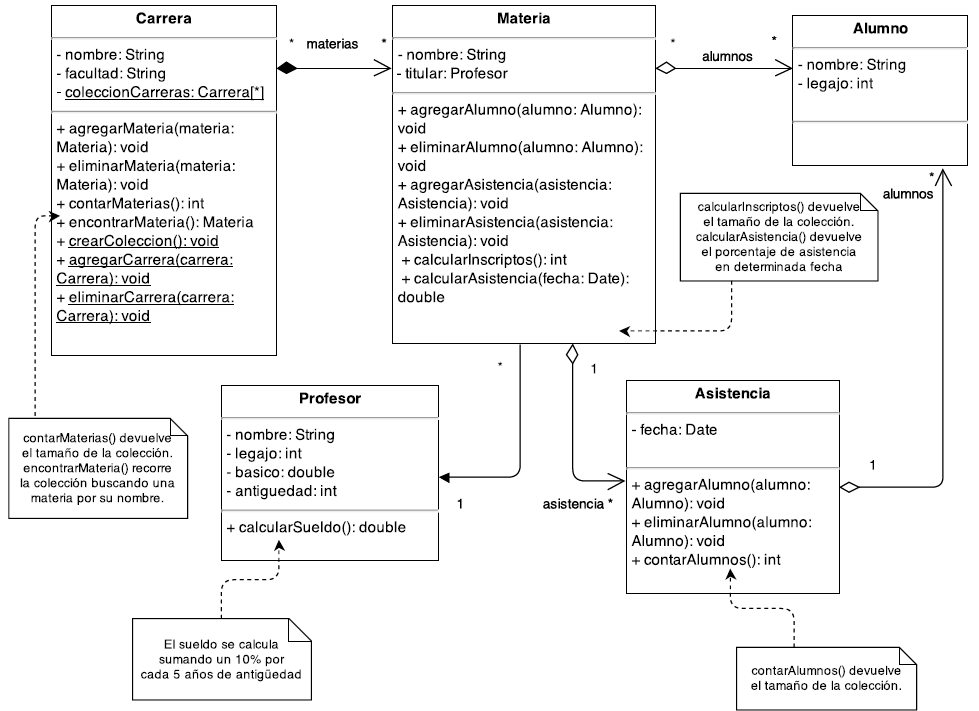
\includegraphics[width=16cm, keepaspectratio]{img/Diagrama-uml.png}
  \caption{Modelo de ejemplo de un diagrama UML.}\label{fig:diagrama-uml}
\end{figure}


\section{Estructura de la memoria}
\label{sec:estructura}

A continuación, describimos la estructura de la memoria, exponiendo el contenido de cada uno de los capítulos, proporcionando así una guía organizada del trabajo de fin de grado para una mejor lectura y comprensión de este.

\begin{itemize}
  
  \item \textbf{Capítulo~\ref{chap:introducción}: Introducción.} En este capítulo se describe en qué consiste el proyecto, la motivación personal que ha llevado a realizarlo y la estructura de la memoria. 

  \item \textbf{Capítulo~\ref{chap:objetivos}: Objetivos.} En este capítulo se establece el objetivo general que se pretende alcanzar con este proyecto. 
  Así como los objetivos específicos necesarios que van a guiar nuestro proyecto y la planificación de dichos objetivos. 
  
  \item \textbf{Capítulo~\ref{chap:estado}: Estado del arte.} En este capítulo se proporciona información detallada sobre el diseño, las características y los usos de cada una de las tecnologías usadas en el proyecto.  
  
  \item \textbf{Capítulo~\ref{chap:diseño}: Diseño e implementación.} En este capítulo se detallan las fases que se han llevado a cabo para realizar el análisis de estudio. 
  También se describe la arquitectura general del proyecto, los procedimientos utilizados para la recolección y el almacenamiento de los datos y la descripción del análisis de los datos.
  %  Discusión de las limitaciones del diseño e implementación??

  \item \textbf{Capítulo~\ref{chap:resultados}: Resultados.} En este capítulo se realiza una descripción detallada de los datos recopilados, de los análisis estadísticos realizados, de los resultados obtenidos en el análisis y ; además, se realiza una conclusión de dichos resultados.
 
  \item \textbf{Capítulo~\ref{chap:conclusiones}: Conclusiones.} En este capítulo se presenta un resumen de los resultados obtenidos y de las conclusiones a las que se ha llegado. 
  También se enumeran los conocimientos adquiridos durante la carrera que se han aplicado en este proyecto y los aprendidos durante la realización de este trabajo.
  Por último, se comentan futuros trabajos o mejoras para el estudio de los desarrolladores que utilizan archivos UML. 
  
  % parte,punto ,apartado
\end{itemize}


%%%%%%%%%%%%%%%%%%%%%%%%%%%%%%%%%%%%%%%%%%%%%%%%%%%%%%%%%%%%%%%%%%%%%%%%%%%%%%%%
%%%%%%%%%%%%%%%%%%%%%%%%%%%%%%%%%%%%%%%%%%%%%%%%%%%%%%%%%%%%%%%%%%%%%%%%%%%%%%%%
% OBJETIVOS %
%%%%%%%%%%%%%%%%%%%%%%%%%%%%%%%%%%%%%%%%%%%%%%%%%%%%%%%%%%%%%%%%%%%%%%%%%%%%%%%%

\cleardoublepage % empezamos en página impar
\chapter{Objetivos} % título del capítulo (se muestra)
\label{chap:objetivos} % identificador del capítulo (no se muestra, es para poder referenciarlo)

En un trabajo de fin de grado es muy importante describir el propósito final del proyecto, definir cuáles serán los aspectos a tratar, así como la planificación llevada a cabo.
Todo esto ayudará a los lectores a hacer un seguimiento del proyecto. 
En este capítulo, se presentan los objetivos del trabajo de fin de grado y los procedimientos planteados para lograrlos.


\section{Objetivo general} % título de sección (se muestra)
\label{sec:objetivo-general} % identificador de sección (no se muestra, es para poder referenciarla)

El objetivo general de este Trabajo Fin de Grado consiste en analizar repositorios de la plataforma GitHub para observar las diferencias y similitudes que existen entre los repositorios que contienen diagramas UML frente al resto de repositorios que no contienen diagramas UML.

\section{Objetivos específicos}
\label{sec:objetivos-especificos}

% Los objetivos específicos se pueden entender como las tareas en las que se ha desglosado el objetivo general.
% relacionados con el planteamiento del problema y el marco teórico, ya que deben responder a las preguntas que se han planteado en la introducción y estar basados en la revisión bibliográfica previa.
% sección crucial para establecer la dirección y los objetivos específicos de la investigación o proyecto, lo que permitirá guiar el trabajo y evaluar su éxito en la consecución de los mismos.
Para lograr el objetivo general de este proyecto se han establecido los siguientes objetivos específicos:

\begin{itemize}
  \item Estudiar y probar el funcionamiento de la herramienta Perceval.
  \item Seleccionar una serie de repositorios de GitHub y almacenar cada uno de ellos en una estructura JSON.
  \item Observar los datos amacenados en los archivos JSON obtenidos e identificar los datos que son de interés para comparar en nuestro estudio.
  \item Desarrollar los programas de extracción y almacenamiento de los datos escogidos en MongoDB.  
  \item Realizar el análisis de los resultados obtenidos para determinar las similitudes y diferencias más relevantes entre los repositorios que tienen archivos UML y los que no.
\end{itemize}


\section{Planificación temporal}
\label{sec:planificacion-temporal}

A finales de abril del año pasado empecé mi proyecto de fin de grado. 
El desarrollo de este trabajo comenzó en mayo de 2022, cuando el profesor Gregorio Robles Martínez me sugirió la idea del proyecto que he llevado a cabo. 


Durante los meses de mayo y junio empecé a documentarme sobre Lindholmen dataset\footnote{\url{http://models-db.com/}}~\cite{robles2017extensive}, que es una base de datos con los repositorios que utilizan diagramas UML en GitHub.
De la misma manera, obtuve la información necesaria sobre las herramientas Grimoire Perceval\footnote{\url{https://github.com/chaoss/grimoirelab-perceval}}~\cite{duenas2018perceval} y GitHub API\footnote{\url{https://docs.github.com/es/rest}}, las cuales se utilizan para analizar repositorios y extraer datos de estos. 
Después del estudio y análisis de estas herramientas, me decanté por Perceval, ya que con ella se obtienen más datos de GitHub.


De julio a septiembre, empecé a descargar y almacenar en MongoDB algunos de los repositorios obtenidos en Lindholmen dataset usando Perceval para ver qué datos se obtenían y cuáles eran más relevantes para, posteriormente, realizar el análisis.
También, inicié el desarrollo de varios programas con los que extaer los datos de interés que, previamente, había seleccionado.


Desde octubre hasta diciembre estuve desarrollando un programa que guardase todos los datos de interés extraídos en MongoDB y otro programa que analizase dichos datos almacenados en MongoDB.
A la vez, fui recopilando y almacenando los datos de una serie de repositorios de desarrolladores en los que hay archivos UML y repositorios en los que no hay archivos UML.
Además, almacené los commits de dichos repositorios; ya que estos contienen información de interés para el desarrollo de nuestro análisis.


Durante los meses de enero y febrero del 2023, busqué cómo introducir los archivos JSON obtenidos, tanto de los repositorios, como de los commits en MongoDB de forma automática, que hasta ese momento había hecho de manera manual.
Esto supuso una mejora en el proceso de desarrollo del proyecto, ya que aceleró la introducción en MongoDB de los datos necesarios para el posterior análisis.
Para ello, decidí crear un programa que ejecutase el proceso de mongoimport de cada uno de los archivos que había descargado. 


Entre marzo y abril, inicié el proceso de escritura de la memoria del proyecto y, a la par, elaboré el programa para analizar los datos obtenidos. 
Por último, durante los meses de mayo y junio desarrollé los programas para la generación de las gráficas con las que visualizar los resultados obtenidos y poder sacar las conclusiones, y finalicé el proceso de redacción de la memoria. 

%%%%%%%%%%%%%%%%%%%%%%%%%%%%%%%%%%%%%%%%%%%%%%%%%%%%%%%%%%%%%%%%%%%%%%%%%%%%%%%%
%%%%%%%%%%%%%%%%%%%%%%%%%%%%%%%%%%%%%%%%%%%%%%%%%%%%%%%%%%%%%%%%%%%%%%%%%%%%%%%%
% ESTADO DEL ARTE %
%%%%%%%%%%%%%%%%%%%%%%%%%%%%%%%%%%%%%%%%%%%%%%%%%%%%%%%%%%%%%%%%%%%%%%%%%%%%%%%%

\cleardoublepage
\chapter{Estado del arte}
\label{chap:estado}

En este capítulo, se presentan las herramientas y librerías usadas en el Trabajo Fin de Grado.
Esta exposición nos da una visión de las tecnologías empleadas en el proyecto.

\section{Tecnologías y herramientas} % título de sección (se muestra)
\label{sec:tecnologías y herramienta}

\subsection{GitHub} % título de sección (se muestra)
\label{sec:github} % identificador de sección (no se muestra, es para poder referenciarla)

GitHub es una plataforma web de desarrollo colaborativo de software\footnote{\url{https://github.com/}} que permite la colaboración y el almacenamiento de proyectos de código abierto o cerrado.
En esta plataforma, los usuarios pueden crear y unirse a proyectos para compartir ideas, discutir posibles soluciones y colaborar entre ellos para mejorar dichos proyecto.
La función principal de GitHub~\cite{astigarraga2022se} es que los usuarios puedan trabajar juntos en un proyecto desde cualquier lugar y en cualquier momento, ya que, registra el desarrollo de los proyectos de forma remota en la nube y no requiere de una infraestructura de hardware específica.
GitHub ofrece una serie de bibliotecas para ayudar a los desarrolladores en su trabajo y herramientas para la gestión de versiones del software, la gestión de problemas, la revisión de código, etc. 
GitHub integra la funcionalidad de Git que es un sistema de control de versiones distribuido.
Se dice que es ``distribuido'' porque git tiene un historial completo de cambios, en el cual se pueden revisar los cambios realizados en el código a lo largo del tiempo. 
Esto permite ver las modificaciones de cada desarrollador e incluso deshacerlas si es necesario. Además permite el trabajo de varios desarrolladores en un mismo proyecto.
En resumen, GitHub es una plataforma que se ha convertido en una herramienta muy popular y esencial en la comunidad de desarrollo de software, ya que permite colaborar y trabajar en equipo para crear proyectos de alta calidad.
 

\subsection{MongoDB} % título de sección (se muestra)
\label{sec:mongodb} % identificador de sección (no se muestra, es para poder referenciarla)

MongoDB\footnote{\url{https://www.mongodb.com/}} es un sistema de gestión de bases de datos no relacional (NoSQL) de código abierto. 
MongoDB ha sido diseñado para almacenar grandes volúmenes de datos; estos datos se almacenan y recuperan en formato BJSON \footnote{\url{https://www.mongodb.com/json-and-bson}} (Binary JSON), en lugar de en un formato de tabla relacional.
El formato BJSON se inventó para solucionar algunos problemas que hacen que usar el formato de representación de objetos JSON no sea la mejor opción dentro de una base de datos. 
Con BJSON se optimiza la velocidad, el espacio y se mejora la eficiencia; solucionando así los problemas que tiene JSON de carecer de soporte para fechas y datos binarios y de no tener una longitud fija para los objetos y las propiedades JSON.
En definitiva, MongoDB es un modelo de base de datos orientado a documentos. Cuando se almacena un documento a éste se le asigna un código que facilita el manejo de los datos que contiene y la recuperación de los mismos.


MongoDB\footnote{\url{https://www.mongodb.com/es/nosql-explained}} tiene un modelo avanzado de consultas e idexación.               
A esto hay que añadir que cuenta con una alta disponibilidad gracias a sus sistemas en la nube y por tanto es capaz de recuperarse en caso de fallo. 
Esta recuperación se consigue mediante el proceso de replicación automática.
La consultas se ejecutan de la siguiente manera: MongoDB recibe por defecto el nodo (index) primario, todas las lecturas y ejecuta todas las escrituras.
El proceso de replicación permite tener siempre una copia exacta del nodo primario, al replicar sus datos en los nodos secundarios.
En el caso de que se produzca un fallo en el sistema, el nodo primario pasaría a ser uno de los secundarios contribuyendo a la recuperación del sistema. 
Otro proceso con el que cuenta es el fragmentación automática (auto-sharding) y el escalado horizontal que permiten la distribución de datos en múltiples servidores de forma que si uno falla, se sustituye rápidamente por otro servidor.
MongoDB también ofrece controles de seguridad integrados para todos los datos.


Por último, MongoDB se puede ejecutar en una variedad de plataformas y sistemas operativos, y es compatible con muchos lenguajes de programación.
Por ello es utilizado en una amplia variedad de aplicaciones, incluyendo aplicaciones web, aplicaciones móviles, juegos y análisis de datos, entre otros.


\subsection{JSON} % título de sección (se muestra)
\label{sec:json} % identificador de sección (no se muestra, es para poder referenciarla)

JSON\footnote{\url{https://www.json.org/json-es.html}} (JavaScript Object Notation) es un formato ligero de intercambio de datos que se utiliza para transmitir y almacenar datos estructurados. 
Fue diseñado con el objetivo de que fuese un formato de texto portátil, mínimo y, originalmente, para ser utilizado con JavaScript. 
JSON es una colección no ordenada de pares clave-valor separados por comas y encerrados en llaves que se puede estructurar como un array o como un objeto~\cite{bray2014javascript}. 
En este proyecto usaremos la estructura JSON de objeto como podemos ver en la figura ~\ref{fig:json}. 


En el siguiente objeto JSON tenemos dos pares clave-valor entre \{ \} y separados por una coma; en los cuales las claves tiene como valor las cadenas ``string1'' y ``string2'' \{``key1'': ``string1'', ``key2'' : ``string2''\}. 
Cada clave es una cadena de caracteres que se identifica con un valor correspondiente; estos valores pueden ser de cualquier tipo de datos: números, cadenas, booleanos, objetos y matrices.
Una de las principales ventajas de JSON es que es fácil de leer y escribir para los humanos, lo que lo hace más fácil de entender y depurar en caso de problemas. 
Este tipo de estructuras son universales y por eso JSON es compatible con la mayoría de los lenguajes de programación y se ha convertido en un formato de datos muy popular.
Por esta razón, al ser tan versátil, se utiliza en aplicaciones web y móviles para transmitir datos entre el cliente y el servidor y como formato para el almacenamiento en bases de datos NoSQL, como MongoDB, Apache Cassandra, y Redis.~\cite{mora2016serializacion}. 

\begin{figure}
  \centering
  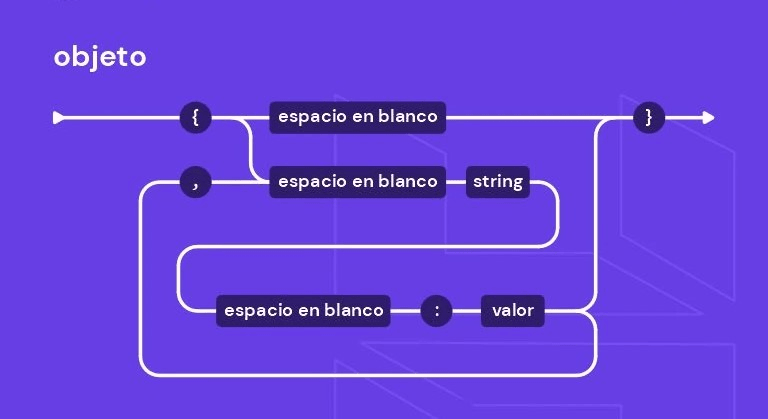
\includegraphics[width=12cm, keepaspectratio]{img/object-json.png}
  \caption{Estructura de un objeto JSON.}\label{fig:json}
\end{figure}

\newpage

\subsection{Python} % título de sección (se muestra)
\label{sec:python} % identificador de sección (no se muestra, es para poder referenciarla)


Python\footnote{\url{https://www.python.org/}} es un lenguaje de programación de alto nivel creado por Guido van Rossum~\cite{challenger2014lenguaje} y lanzado por primera vez en 1991, cuyo nombre está inspirado en el grupo de cómicos “Monty Python”.  


Fue diseñado para facilitar la escritura de código y por tanto destaca por ser un lenguaje potente, sencillo, fácil de aprender y con una sintaxis clara y legible.
Se considera un lenguaje multiparadigma, ya que, se apoya en diferentes estilos de programación como la programación orientada a objetos, la programación funcional y la programación imperativa.   
Python además cuenta con estructuras de datos para facilitar el desarrollo de software como listas, diccionarios, conjuntos y tuplas.
También tiene una gran cantidad de bibliotecas y herramientas que facilitan el desarrollo de software; ya que, con ellas se obtienen soluciones en la tareas básicas de un programador.


Además, Python~\cite{rios2016evaluacion} cuenta con un intérprete propio y tiene compatibilidad con diferentes plataformas y sistemas operativos al ser un lenguaje de código abierto.
Esta es una de las razones de que sea utilizado en una amplia variedad de aplicaciones, como el desarrollo web, el análisis de datos, la inteligencia artificial, el aprendizaje automático, la automatización de tareas y la creación de juegos, entre otros.
Por todo esto, este lenguaje ha ganado mucha fuerza en la comunidad científica, educacional y de sofware libre.


\subsection{Ubuntu} % título de sección (se muestra)
\label{sec:ubuntu} % identificador de sección (no se muestra, es para poder referenciarla)

Ubuntu\footnote{\url{https://ubuntu.com/}} es un sistema operativo de código abierto basado en Linux diseñado con una gran cantidad de software preinstalado para satisfacer las necesidades de la mayoría de los usuarios.
Fue lanzado por primera vez en 2004 y desarrollado por una empresa llamada Canonnical~\cite{martinez2006software}, cuyo objetivo era generar un sistema fácil de instalar y utilizar, completo e innovador. 


Actualmente Ubuntu~\cite{tavera2013software} se ha convertido en uno de los sistemas operativos más populares en la comunidad de software libre y de código abierto.
Esto se debe a que está disponible de forma gratuita para su descarga y uso de múltiples formas y, además, tiene una interfaz muy parecida a Windows lo que permite que sea intuitivo y fácil de utilizar por cualquier usuario.


Al igual que con Windows, con este sistema operativo también podemos navegar en la web, crear y modificar documentos, al ser compatible con formatos de archivos muy conocidos, y otras tareas que realizamos en nuestro día a día. 
Ubuntu se utiliza en una amplia variedad de sistemas, desde ordenadores hasta servidores y dispositivos móviles. 

\subsection{WSL} % título de sección (se muestra)
\label{sec:wsl} % identificador de sección (no se muestra, es para poder referenciarla)

WSL\footnote{\url{https://learn.microsoft.com/es-es/windows/wsl/}}(Windows Subsystem for Linux) es un sistema diseñado por Microsoft que permite a los desarrolladores ejecutar aplicaciones y herramientas de línea de comandos de Linux directamente en Windows, sin necesidad de utilizar una máquina virtual o instalar un sistema operativo Linux en un disco duro. 
Este subsistema de Windows para Linux fue lanzado en 2016 y no ha dejado de evolucionar desde entonces. 


WSL~\cite{medriforensic} fue creado para los desarrolladores que necesitan utilizar herramientas y aplicaciones de línea de comandos específicas de Linux, pero prefieren trabajar en el entorno de Windows. 
También para aquellos que necesitan trabajar en los sistemas operativos Windows y Linux simultáneamente.


La versión WSL 1 utiliza una capa de compatibilidad para la transferencia de la ejecución de código entre Windows y Linux;
mientras que WSL 2 tiene una versión actualizada de su arquitectura del software con respecto a su versión anterior. 
Además, utiliza una máquina virtual de Linux integrada que ofrece un rendimiento alto y muy parecido al de un sistema Linux real.


\subsection{LaTex} % título de sección (se muestra)
\label{sec:latex} % identificador de sección (no se muestra, es para poder referenciarla)

LaTeX\footnote{\url{https://es.overleaf.com/}} es un sistema de composición de textos o documentos formado por un conjunto de macros TeX. 
Fue desarrollado por Leslie Lamport en 1984, con el fin de facilitar el uso del lenguaje de composición tipográfica de textos TeX.
TeX es, también, un sistema de composición tipográfica de textos que usa funciones avanzadas de automatización para generar documentos en los cuales se usan textos y fórmulas matemáticas con un determinado estándar.
Fue desarrollado por Donald E. Knuth en 1978 como herramienta para la creación de textos que contengan fórmulas matematicas complejas.


LaTeX~\cite{rodriguez2014edicion} usa las características del sistema TeX para generar documentos científicos, técnicos y académicos de alta calidad automáticamente, como artículos académicos, libros, tesis, informes, etc.   
Además, LaTeX ofrece con una variedad de paquetes, extensiones y estilos personalizados para adaptarse a las indicaciones específicas de cada usuario.
Las extensiones con las que cuenta permiten insertar fácilmente imágenes, diagramas matemáticos, fórmulas matemáticas, textos de lenguajes de programación, etc.


Estos sistemas de composición de textos están disponibles en gran cantidad de plataformas; además, cuentan con editores gratuitos que facilitan la creación de documentos sin la necesidad de tener conocimientos previos de programación.
LaTeX utiliza una sintaxis de comandos que permiten al usuario controlar la estructura y el formato del documento, incluyendo la disposición de los elementos, el estilo de las fuentes, las ecuaciones matemáticas, y las referencias bibliográficas. 


Una vez que se domina la sintaxis y las herramientas de LaTeX, se puede crear fácilmente documentos de alta calidad de manera eficiente.
Por eso LaTeX es una herramienta muy utilizada y valorada en la comunidad científica, técnica y académica; y se utiliza ampliamente en universidades y centros de investigación de todo el mundo por su capacidad para producir documentos de alta calidad con un aspecto profesional, incluso si se requiere un formato complejo y detallado. 


\section{Librerías} % título de sección (se muestra)
\label{sec:librerías}

\subsection{Perceval} % título de subsección (se muestra)
\label{sec:perceval} % identificador de subsección (no se muestra, es para poder referenciarla)


Perceval\footnote{\url{https://github.com/chaoss/grimoirelab-perceval}} es uno de los componentes que contiene GrimoireLAb\footnote{\url{https://chaoss.github.io/grimoirelab/}}, que es uno de los proyectos fundadores de CHAOSS Software\footnote{\url{https://chaoss.community/}}.
Este proyecto fue desarrollado para ayudar a investigadores en el análisis de repositorios de software y está formado por un conjunto de herramientas gratuitas, libres y de código abierto. 


GrimoireLAb es el resultado de más de 10 años de desarrollo de Bitergia, empresa que emergió del grupo de investigación de software libre de la URJC y varios colaboradores. 
Cada herramienta se encuentra disponible en un repositorio distinto en GitHub y se puede instalar fácilmente como un módulo de paquetes de Python.
Dichas herramientas se crearon para la recopilación automática e incremental de información de cualquier fuente de datos, el enriquecimiento de estos con información adicional y el almacenamiento y visualización de estos datos. 


GrimoireLAb cuenta con unos componentes que se pueden usar juntos o por separado para las distintas tareas que se ejecutan en un análisis de datos.  
Perceval, como ya hemos mencionado, es uno de estos componentes que funciona como una biblioteca/módulo y proporciona una API de Python.
Está diseñado para recuperar datos relacionados con el desarrollo de software de diferentes fuentes.
Estas fuentes pueden ser de gestión de problemas o tareas, de gestión o revisión de código fuente, de foros o listas de correo, de wikis, entre otros.
Posteriormente, se guarda la información obtenida en una base de datos en un formato estandarizado.
Los datos que obtenemos con Perceval se almacenan como diccionarios de Python o como documentos JSON como el que mostramos a continuación: 

{\footnotesize
\begin{verbatim}
  {
    "backend_name": "GitHub",
    "backend_version": "0.2.2",
    "data": {
    ...
    },
    "origin": "https://github.com/grimoirelab/perceval",
    "perceval_version": "0.1.0",
    "timestamp": 1476139775.852378,
    "updated_on": 1451929343.0,
    "uuid": "c403532b196ed4020cc86d001feb091c009d3d26"
  }
\end{verbatim}
}

Esta herramienta es muy útil para desarrolladores, analistas de datos y cualquier persona interesada en la recuperación de información de diferentes fuentes de datos y su posterior análisis.
Además, cualquier persona puede participar en este proyecto aportando soluciones para corregir errores o ideas para nuevos servicios o funciones.
También, cuenta con una comunidad de desarrolladores que colaboran continuamente en el mantenimiento y la actualización de sus servicios. 

\subsection{Pymongo} % título de subsección (se muestra)
\label{sec:pymongo} % identificador de subsección (no se muestra, es para poder referenciarla)

Pymongo\footnote{\url{https://pypi.org/project/pymongo/}} es una librería de Python que contiene varias herramientas con las que podemos interactuar fácilmente desde un archivo de Python con MongoDB, siendo éste una base de datos NoSQL. 
Con PyMongo, se pueden realizar una variedad de tareas en MongoDB, como crear y eliminar bases de datos y colecciones, insertar, actualizar y eliminar documentos, realizar consultas y filtrar datos, entre otras posibilidades.
% PyMongo proporciona una API completa y fácil de usar para realizar operaciones de CRUD (crear, leer, actualizar y eliminar) en MongoDB desde Python. 


\subsection{Subprocess} % título de subsección (se muestra)
\label{sec:subprocess} % identificador de subsección (no se muestra, es para poder referenciarla)
El módulo ``subprocess''\footnote{\url{https://docs.python.org/es/3/library/subprocess.html}} (subproceso) permite ejecutar un proceso que se encuentra dentro de un script de Python a la vez que se ejecuta dicho script.
Esto es posible gracias a que este módulo interactúa con el sistema operativo haciendo posible ejecutar y administrar subprocesos directamente desde Python. 
Este módulo proporciona varias funciones y clases para interactuar con procesos externos con los cuales los desarrolladores pueden ejecutar comandos en la línea de comandos del sistema operativo y manipular la entrada y salida de estos procesos.

\subsection{Mongoimport} % título de subsección (se muestra)
\label{sec:mongoimport} % identificador de subsección (no se muestra, es para poder referenciarla)

\emph{Mongoimport}\footnote{\url{https://www.mongodb.com/docs/database-tools/mongoimport/}} es una herramienta que forma parte del paquete ``MongoDB Database Tools''
Esta herramienta se utiliza para importar datos de archivos en formato JSON, CSV o TSV con facilidad desde la línea de comandos a una base de datos MongoDB. 
Con \emph{mongoimport}, se pueden importar grandes cantidades de datos de manera eficiente, además, se permite especificar la base de datos y la colección en la que se quieren almacenar.
El comando que se ha usado para importar los archivos es el siguiente:

\begin{verbatim}
mongoimport --db nombre_base_datos --collection nombre_coleccion
--file dirección_archivo_a_importar
\end{verbatim}

\subsection{Matplotlib} % título de subsección (se muestra)
\label{sec:matplotlib} % identificador de subsección (no se muestra, es para poder referenciarla)

Matplotlib\footnote{\url{https://matplotlib.org/}} es una librería de código abierto de Python que se usa para crear gráficos estadísticos, figuras interactivas, coordenadas no estructuradas, gráficos 3D y otros tipos de visualización de datos.
Esta librería proporciona una amplia gama de herramientas; la mayoría se ofrecen como funciones del módulo ``pyplot'', pero también integra otras librerías de Python como NumPy y Pandas, que facilita el trabajo con grandes conjuntos de datos y su visualización.
Gracias a todas estas herramientas, Matplotlib permite crear gráficos de alta calidad con una sintaxis simple, por lo que se ha convertido en una opción muy popular para la generación de gráficas.


Como hemos mencionado, Matplotlib utiliza el módulo Pyplot\footnote{\url{https://matplotlib.org/stable/tutorials/introductory/pyplot.html}} que fue diseñado para la generación de gráficos programáticos e interactivos.
Este módulo proporciona una interfaz sencilla, semejante a la de Matlab, que además ofrece una representación de gráficas implícita.
También es importante destacar que el módulo de ``pyplot'' tiene un conjunto de funciones sencillas con las cuales se pueden crear gráficos y personalizarlos (trazar líneas, añadir elementos, textos, etiquetas, etc.) adaptándolos a los requisitos que tenga cada usuario. 

 
\subsection{Numpy} % título de subsección (se muestra)
\label{sec:numpy} % identificador de subsección (no se muestra, es para poder referenciarla)

NumPy\footnote{\url{https://numpy.org/}} es una librería de código abierto de Python que permite realizar cálculos numéricos y operaciones matemáticas de manera eficiente.
Esta librería consta de una gran conjunto de herramientas y funciones matemáticas que realizan operaciones con matrices multidimensionales y operaciones de alto nivel.  


%%%%%%%%%%%%%%%%%%%%%%%%%%%%%%%%%%%%%%%%%%%%%%%%%%%%%%%%%%%%%%%%%%%%%%%%%%%%%%%%
%%%%%%%%%%%%%%%%%%%%%%%%%%%%%%%%%%%%%%%%%%%%%%%%%%%%%%%%%%%%%%%%%%%%%%%%%%%%%%%%
% DISEÑO E IMPLEMENTACIÓN %
%%%%%%%%%%%%%%%%%%%%%%%%%%%%%%%%%%%%%%%%%%%%%%%%%%%%%%%%%%%%%%%%%%%%%%%%%%%%%%%%

\cleardoublepage
\chapter{Diseño e implementación}
\label{chap:diseño}

A continuación, describiremos los métodos y herramienta utilizados para llevar a cabo el trabajo. 
Esto permite a los lectores entender cómo se ha desarrollado el proyecto para realizar el análisis de estudio.
En este capítulo se detallan las fases del proyecto, las decisiones y justificaciones de las metodologías escogidas y el diseño e implementación para que otros puedan realizar el mismo análisis.

\section{Proceso} 
\label{sec:proceso}

En la figura~\ref{fig:arquitectura} se observan las fases en las cuales se divide este proyecto\footnote{\url{https://github.com/carmengl98/extraccion_analisis_repos}}. 
En la primera fase se realiza la recopilación de datos de GitHub mediante la herramienta de Perceval\footnote{\url{https://perceval.readthedocs.io/en/latest/perceval/perceval-backends.html}}. 
Esta herramienta nos permite conectarmos a la API de GitHub para extraer los datos en documentos JSON con la información de los repositorios y los commits realizados en estos mismos repositorios.
Perceval~\cite{duenas2018perceval} cuenta con una estructura formada por tres componentes que interactuan entre ellos para facilitar la recuperación de datos de diferentes fuentes de desarrollo de software.
A continuación, vamos a describir cómo funciona la interacción entre los componentes de esta estructura.


``The CommandLine'' o la línea de comandos es uno de los componentes de Perceval que permite a los usuarios interactuar con esta herramienta.
A través de la línea de comandos se especifica el backend con el cual se va a interactuar, además se pueden especificar el tipo de fuentes de datos, opciones de configuración e incluir argumentos para personalizar la recuperación de datos como filtros de fecha, límite de elementos a recuperar, configuraciones de salida, entre otras.
Estos argumentos adicionales brindan a los usuarios mayor flexibilidad y control al utilizar el backend a través de la interfaz de línea de comandos, permitiéndoles personalizar aún más la forma en que interactúan con Perceval.


Otro de los componentes es el ``cliente'' que se encarga de interpretar los argumentos y opciones de configuración proporcionadas a través de la línea de comandos y de gestionar la interacción entre esta y el backend correspondiente.
Este también es responsable de manejar tanto las complicaciones asociadas a la consulta de la fuente de datos como los problemas de conexión con fuentes de datos remotas y ofrecer soluciones específicas en caso de ser necesarias.
 

El tercer y último componente es el ``backend'' que se encarga de organizar la implementación de mecanismos incrementales y de almacenamiento en caché para mejorar la eficiencia y la velocidad de recopilación de una fuente de datos específica.
Perceval ofrece varios backend diseñados para adaptarse a los requisitos específicos de cada fuente de datos correspondiente; sin embargo estos backends tienen características comunes como la incrementalidad y el almacenamiento en caché.


Después de extraer ficheros JSON de GitHub con Perceval, introduciremos los datos de los commits realizados en los repositorios en MongoDB mediante la librería ``subprocess'' de Python que realiza una llamada al comando ``mongoimport'' e introduce cada uno de los archivos JSON.
Una vez introducidos usamos un scrpit creado para modificar los documentos JSON obtenidos de los repositorios.
Este script recorre la estructura de los documentos JSON y añade varios campos a esta estructura JSON: los datos extraídos de cada uno de los commits que se han realizado en cada repositorio, el número total de commits en el repositorio, un booleano que nos indica si el repositorio contiene diagramas UML o no, los colaboradores que han realizado commits en los repositorios y el número de estos colaboradores.
Posteriormente, se introduccen estos nuevos documetos JSON en MongoDB.


En la segunda fase procesaremos cada uno de los archivos JSON, antes de almacenarlos en la base de datos MongoDB, de tal forma que nos quedemos con los datos que nos interesan para el análisis que vamos a realizar y descartemos el resto de datos.
Por último, realizaremos un análisis estadístico de los datos recopilados. 

\begin{figure}
  \centering
  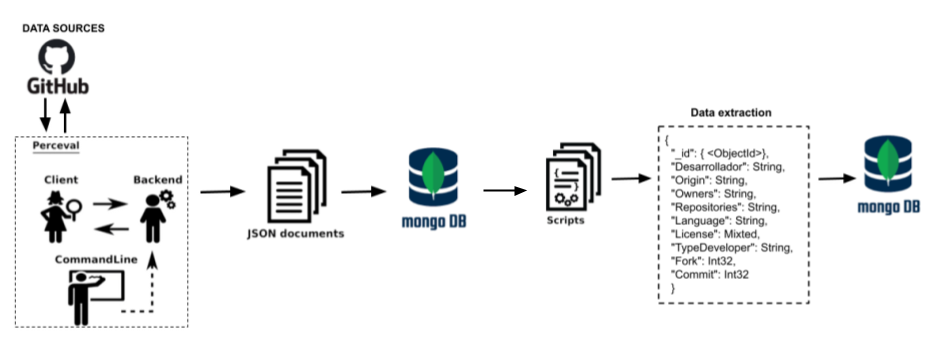
\includegraphics[width=17cm, keepaspectratio]{img/Arquitectura_general.png}
  \caption{Descripción del proceso de extracción y filtrado de datos.}\label{fig:arquitectura}
\end{figure}


\section{Procedimiento de instalación} % título de sección (se muestra)
\label{sec:procedimiento de instalación}

Para poder realizar este proyecto es necesario tener intalados WSL (Windows Subsystem for Linux) en Windows y, en dicho Subsistema de Windows, tener Ubuntu como sistema operativo, además de la librería Perceval. 
A continuación, procederemos a explicar los pasos a seguir para realizar correctamente las instalaciones necesarias.

\subsection{Instalación de WSL} % título de sección (se muestra)
\label{sec:instalación de WSL}

En primer lugar, comprobaremos que nuestro ordenador cumple con los requisitos previos a la instalación, ya que para instalar WSL se necesita tener Windows 10 versión 2004 o posterior y nuestro hardware debe ser compatible con la virtualización de Hyper-V. 


Para verificar la versión de Windows, se debe abrir la Configuración y después seleccionar ``Sistema'' y, por último hacer clic en ``Acerca de''.


Para comprobar si nuestro procesador es compatible con Hyper-V debemos ir al menú de inicio de Windows y buscar ``Información del sistema''.

\begin{figure}
  \centering
  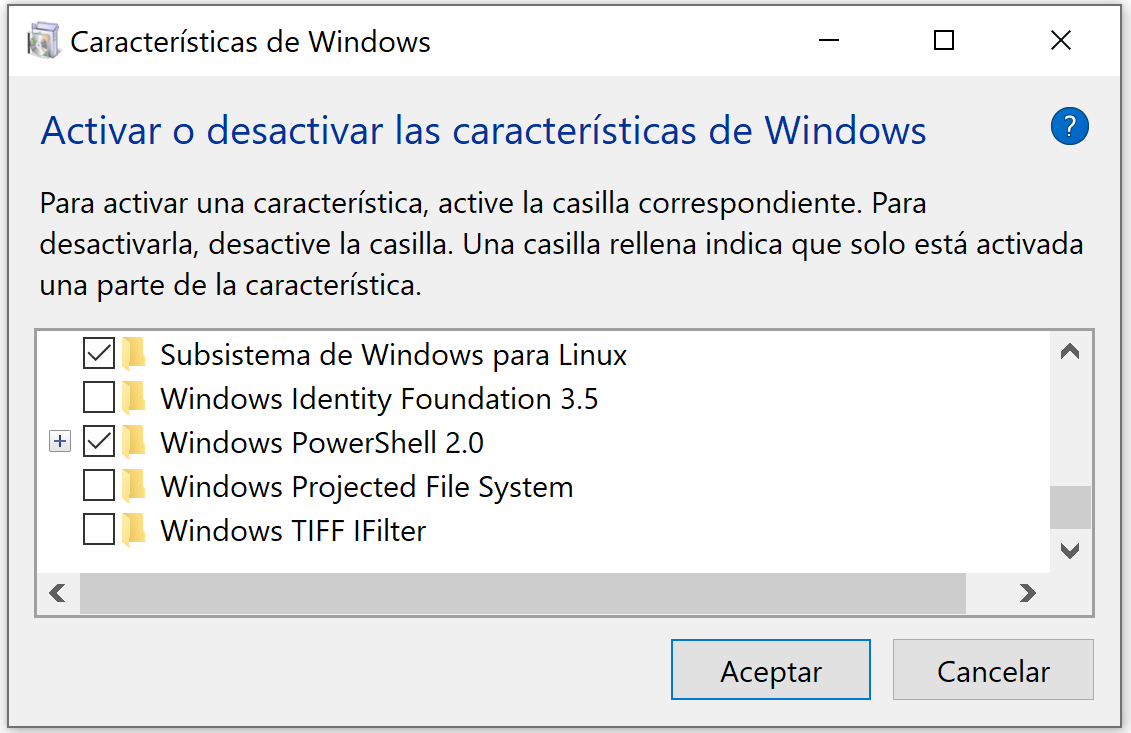
\includegraphics[width=10cm, keepaspectratio]{img/CaracteristicasWindows.PNG}
  \caption{Características de Windows.}\label{fig:CaracteristicasWindows}
\end{figure}


Si cumplimos estos requisitos, lo primero que tenemos que hacer es activar los permisos para que en Windows se pueda usar WSL.
Para habilitar los permisos para usar WSL en Windows debemos seguir los siguientes pasos:
\begin{enumerate}
  \item Ir al menú de inicio de Windows y buscar ``Activar o desactivar las características de Windows''.
  \item Marcar la casilla de verificación de ``Subsistema de Windows para Linux'' como podemos observar en la figura~\ref{fig:CaracteristicasWindows}.
  \item Hacer clic en ``Aceptar'' y esperar a que finalice el proceso. 
  \item Por último, reiniciar el ordenador para completar la instalación.
\end{enumerate} 
  

Una vez que nos aseguremos de cumplir estos requisitos y tener habilitado WSL en el ordenador procedemos a instalar la distribución de Linux (Ubuntu) desde la Microsoft Store para usar en WSL. 

\subsection{Instalación de Ubuntu} % título de sección (se muestra)
\label{sec:instalación de ubuntu}

A continuación, descargaremos la versión de GNU/Linux que queramos usar, en nuestro caso hemos descargado la versión Ubuntu 20.04.5 LTS.


Desde la propia tienda de aplicaciones de Windows debemos buscar ``Ubuntu'', seleccionar la versión deseada y hacer clic en ``Obtener'', como mostramos en la figura~\ref{fig:ubuntu}.
Cuando se ha descargado podremos comprobar que Ubuntu se ejecuta con WSL.

\begin{figure}
  \centering
  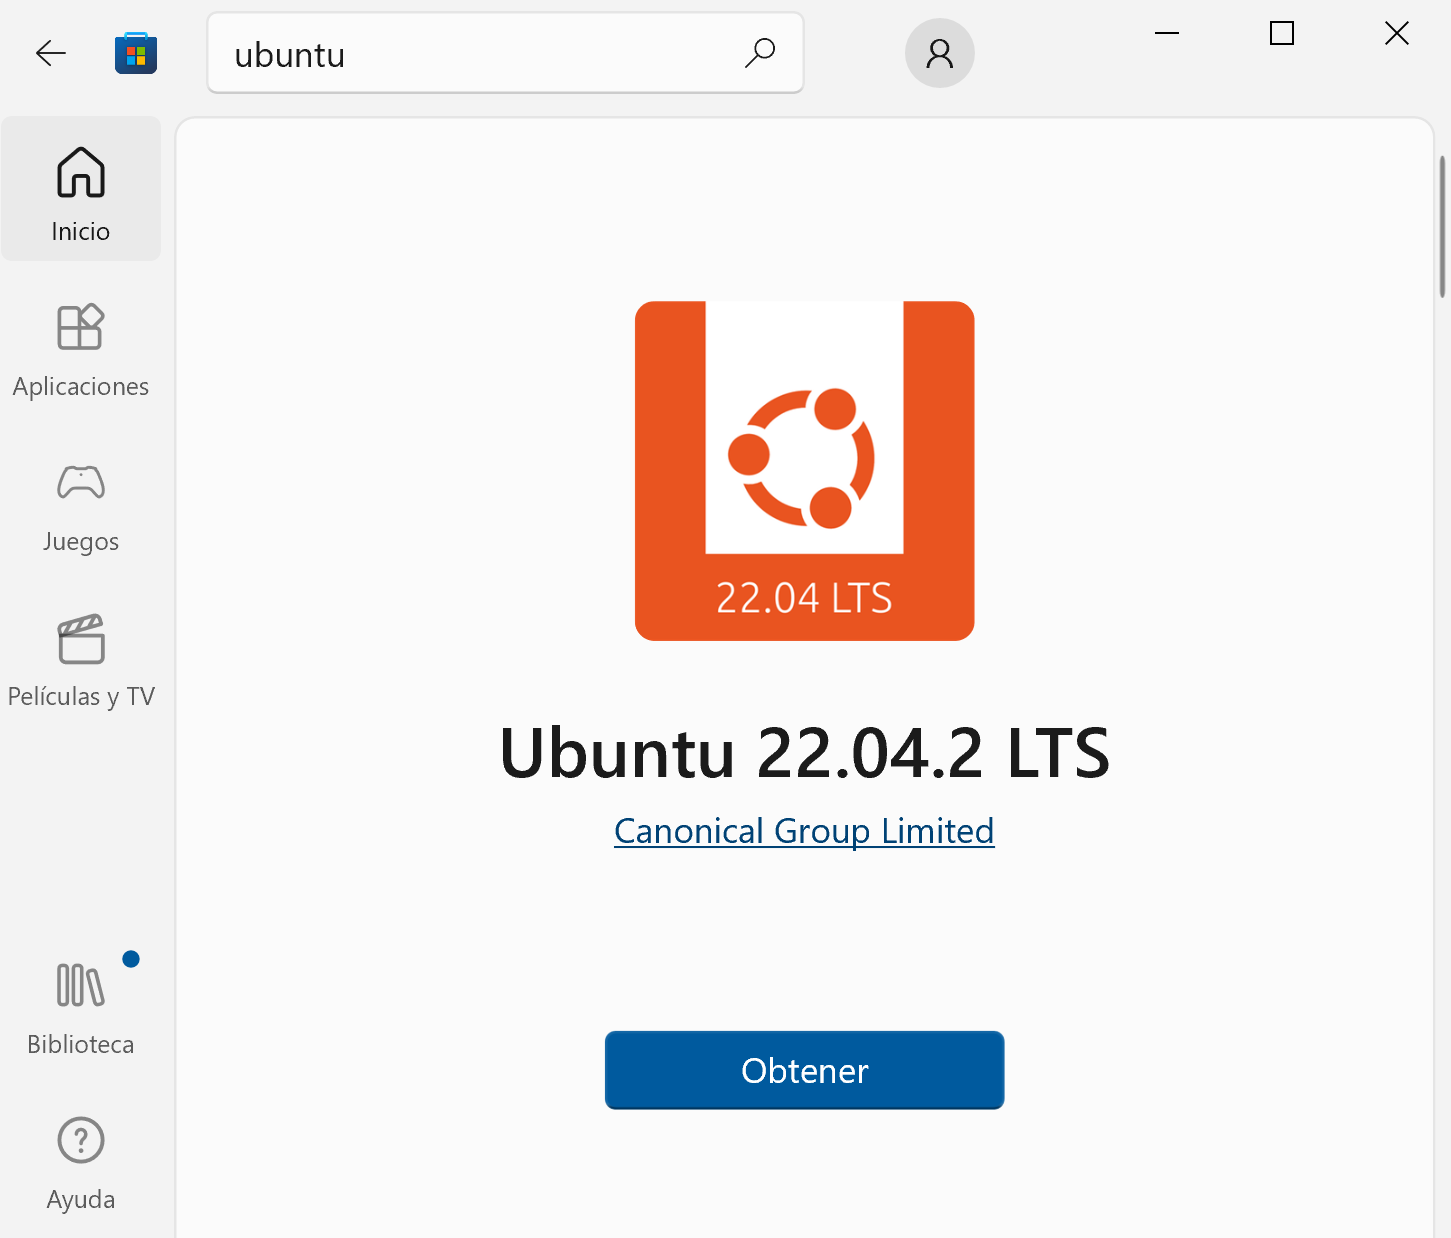
\includegraphics[width=10cm, keepaspectratio]{img/Ubuntu.PNG}
  \caption{Características de Windows.}\label{fig:ubuntu}
\end{figure}

\subsection{Instalación de Perceval} % título de sección (se muestra)
\label{sec:instalación de perceval}

Antes de instalar Perceval tenemos que conectarnos al Subsistema de Windows para Linux ya que instalaremos dicha librería en este entorno.
A continuación, para acceder a WSL abriremos Visual Studio Code e instalaremos la extensión WSL que vemos en la figura~\ref{fig:extensionwsl}, que permite obtener toda la productividad de Windows mientras se trabaja con las herramientas y utilidades basadas en Linux.
Con esta extensión se puede utilizar VS Code en WSL tal y como se haría desde Windows.

\begin{figure}
  \centering
  
\includegraphics[width=14cm, keepaspectratio]{img/extension_wsl.PNG}
  \caption{Estencion WSL de Visual Studio Code.}\label{fig:extensionwsl}
\end{figure}

Una vez estemos conectados a WSL, pasamos a realizar los siguientes pasos para instalar Perceval en Ubuntu:
\begin{enumerate}
  \item Instalar la última versión de Python y Pip, si aún no se tiene instalada en el sistema.
  \item Instalar las dependencias requeridas para GrimoireLab Perceval utilizando el siguiente comando: \emph{pip install perceval}
\end{enumerate}

Para verificar que la instalación se ha completado con éxito usaremos el comando \emph{perceval --version}. 
Si este comando devuelve la versión de GrimoireLab Perceval instalada, entonces la instalación se ha completado correctamente y se puede empezar a utilizar Perceval para recopilar datos de diversas fuentes de software.

\section{Recopilación de datos} % título de sección (se muestra)
\label{sec:recopilación de datos}

En esta parte del proyecto se lleva a cabo la recopilación de una lista de repositorios que utilizan archivos UML y otra en las que no se utilizan archivos UML.
Para ello se recurre al Lindholmen dataset que proporciona a los investigadores listas de proyectos de código abierto que usan archivos UML y que se encuentran distribuidos en repositorios de GitHub.

A partir de este conjunto de datos se descarga el archivo ``UMLFilesList'' para obtener una lista de los repositorios que hacen uso de archivos UML.
Este archivo proporciona los enlaces directos a los archivos UML de cada uno de los repositorios, lo que permite verificar que dichos archivos siguen formando parte de dichos repositorios.
Con estos enlaces nos cercioramos de que los archivos continuen, cada uno de ellos, siendo parte de los diferentes proyectos, que posteriormente procederemos a analizar. 


Para obtener la lista de repositorios en los que no se usen archivos UML se procede a revisar los seguidores de los repositorios obtenidos anteriormente y se selecionan de forma aleatoria algunos de ellos para crear dicha lista.


Una vez que se obtienen ambas listas de repositorios, se procede a descargar los datos de los mismos, así como los de los commits, empleando la herramienta Grimoire Perceval.
Esta herramienta soporta más de 30 fuentes de datos de los cuales se pueden obtener datos.
En la figura ~\ref{fig:perceval-json} vemos un esquema del procedimiento que sigue Perceval. 
En éste, el cliente escoge la fuente de la cual desea obtener los datos a analizar y ejecuta Perceval desde la línea de comandos con los parámetros necesarios para recopilar la información de la fuente seleccionada.
Posteriormente, Perceval procesa esta información y la almacena en documentos. 

\begin{figure}
  \centering
  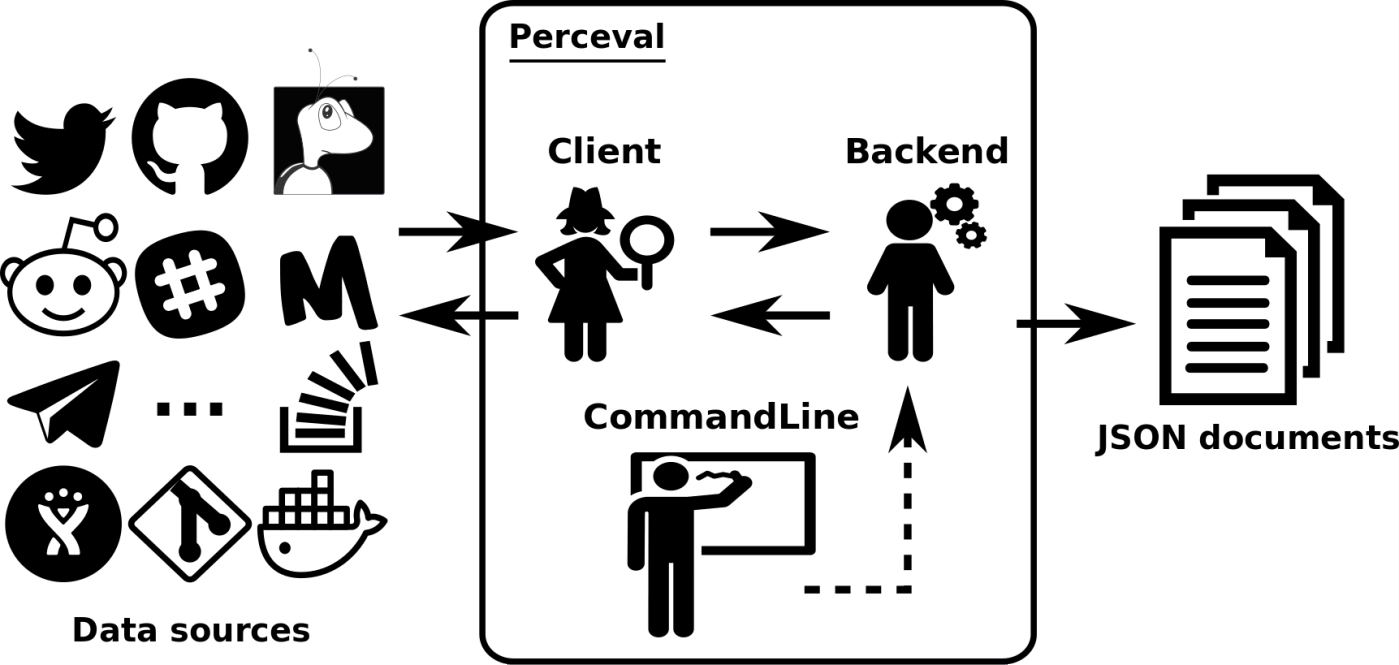
\includegraphics[width=12cm, keepaspectratio]{img/perceval-json.png}
  \caption{Descripción general de Perceval.}\label{fig:perceval-json}
\end{figure}

En este proyecto se eligió como fuente de datos GitHub. 
Partiendo de esta fuente de datos se le pasaron a Perceval los siguientes parámetros: el nombre del repositorio o dirección URL, el nombre y tipo de archivo con el que queremos que se guarden los documentos generados y, además, según el comando usado obtendremos los datos de los repositorios o de otras categorías como, en este caso, los commits, u otras como las issues, los pull request, etc.
\begin{verbatim}
perceval github --category repository grimoirelab Perceval > repo.json
perceval git https://github.com/grimoirelab/perceval.git > commit.json
\end{verbatim} 
    

Gracias a esta herramienta, se pudo obtener información detallada de los repositorios y los commits, lo que resultó fundamental para el desarrollo de este proyecto de investigación.
Estos datos se guardaron en archivos JSON, puesto que es una estructura de datos ampliamente utilizada y fácil de comprender.
Para llevar a cabo esta tarea usamos una conexion WLS en la que se instaló tanto Ubuntu como la librería de Perceval; ya que en Windows daba problemas.
La intalación tanto de WLS como de Ubuntu y Perceval se han explicado en el apartado ~\ref{sec:procedimiento de instalación}.

Después de finalizar el proceso de obtención de los datos de los repositorios se procedió a almacenarlos en la base de datos MongoDB.
Para este fin, se buscó una forma de introducir los archivos JSON de forma automática. 
Para ello, se uso el módulo de python \emph{subprocess} junto con \emph{mongoimport} para desarrollar los ficheros que introducen todos los documentos JSON, obtenidos anteriormente, para crear la base de datos que vamos a estudiar.
En estos ficheros se ejecuta \emph{mongoimport} con cada uno de los archivos JSON obtenidos, tanto de los de los repositorios como de los commits con el comando que se muestra a continuación:
\begin{verbatim}
  mongoimport --db project --collection Repositories --file
   "...\repository\repoFile.json"
  mongoimport --db project --collection Commits --file 
  "...\commit\commitFile.json"
\end{verbatim}


en el cual;
\begin{itemize}
  \item ``Project'' es el nombre de nuestra base de datos
  \item ``Repositories'' es el nombre de la colección en la que almacenaremos todos los datos extraídos de cada repositorio.
  \item ``Commits'' es el nombre de la colección en la que almacenaremos todos los datos extraídos de cada commit hecho por cada repositorio.
  \item ``...\textbackslash repository\textbackslash repoFile.json'' es la ruta en la que se encuentran todos los archivos JSON que se corresponden con los datos extraídos de los repositorios.
  \item  ``...\textbackslash commit\textbackslash commitFile.json'' es la ruta en la que se han almacenado los archivos JSON con los datos de los commits generados por los repositorios
\end{itemize}

\section{Procesado de datos} % título de sección (se muestra)
\label{sec:procesado de datos}

Después de almacenar todos los archivos JSON de la lista de respositorios seleccionados, empezamos a observar los datos obtenidos y se eligieron los más adecuados para analizar los tipos de desarrolladores seleccionados. 
Posteriormente, se inició el desarrollo de varios ficheros con los que extaer los datos de mayor interés. 
Al mismo tiempo, se estudió en qué tipo de base de datos se deberían guardar los archivos JSON obtenidos con Perceval.
Se optó por una base de datos que no fuese relacional (NoSQL), ya que este tipo de bases de datos son muy útiles para trabajar con grandes conjuntos de datos distribuidos y soportan cargas de trabajo intensas.
Por esta razón, se decidió almacenarlos en MongoDB que es una base de datos NoSQL de código abierto. 

\begin{figure}
  \centering
  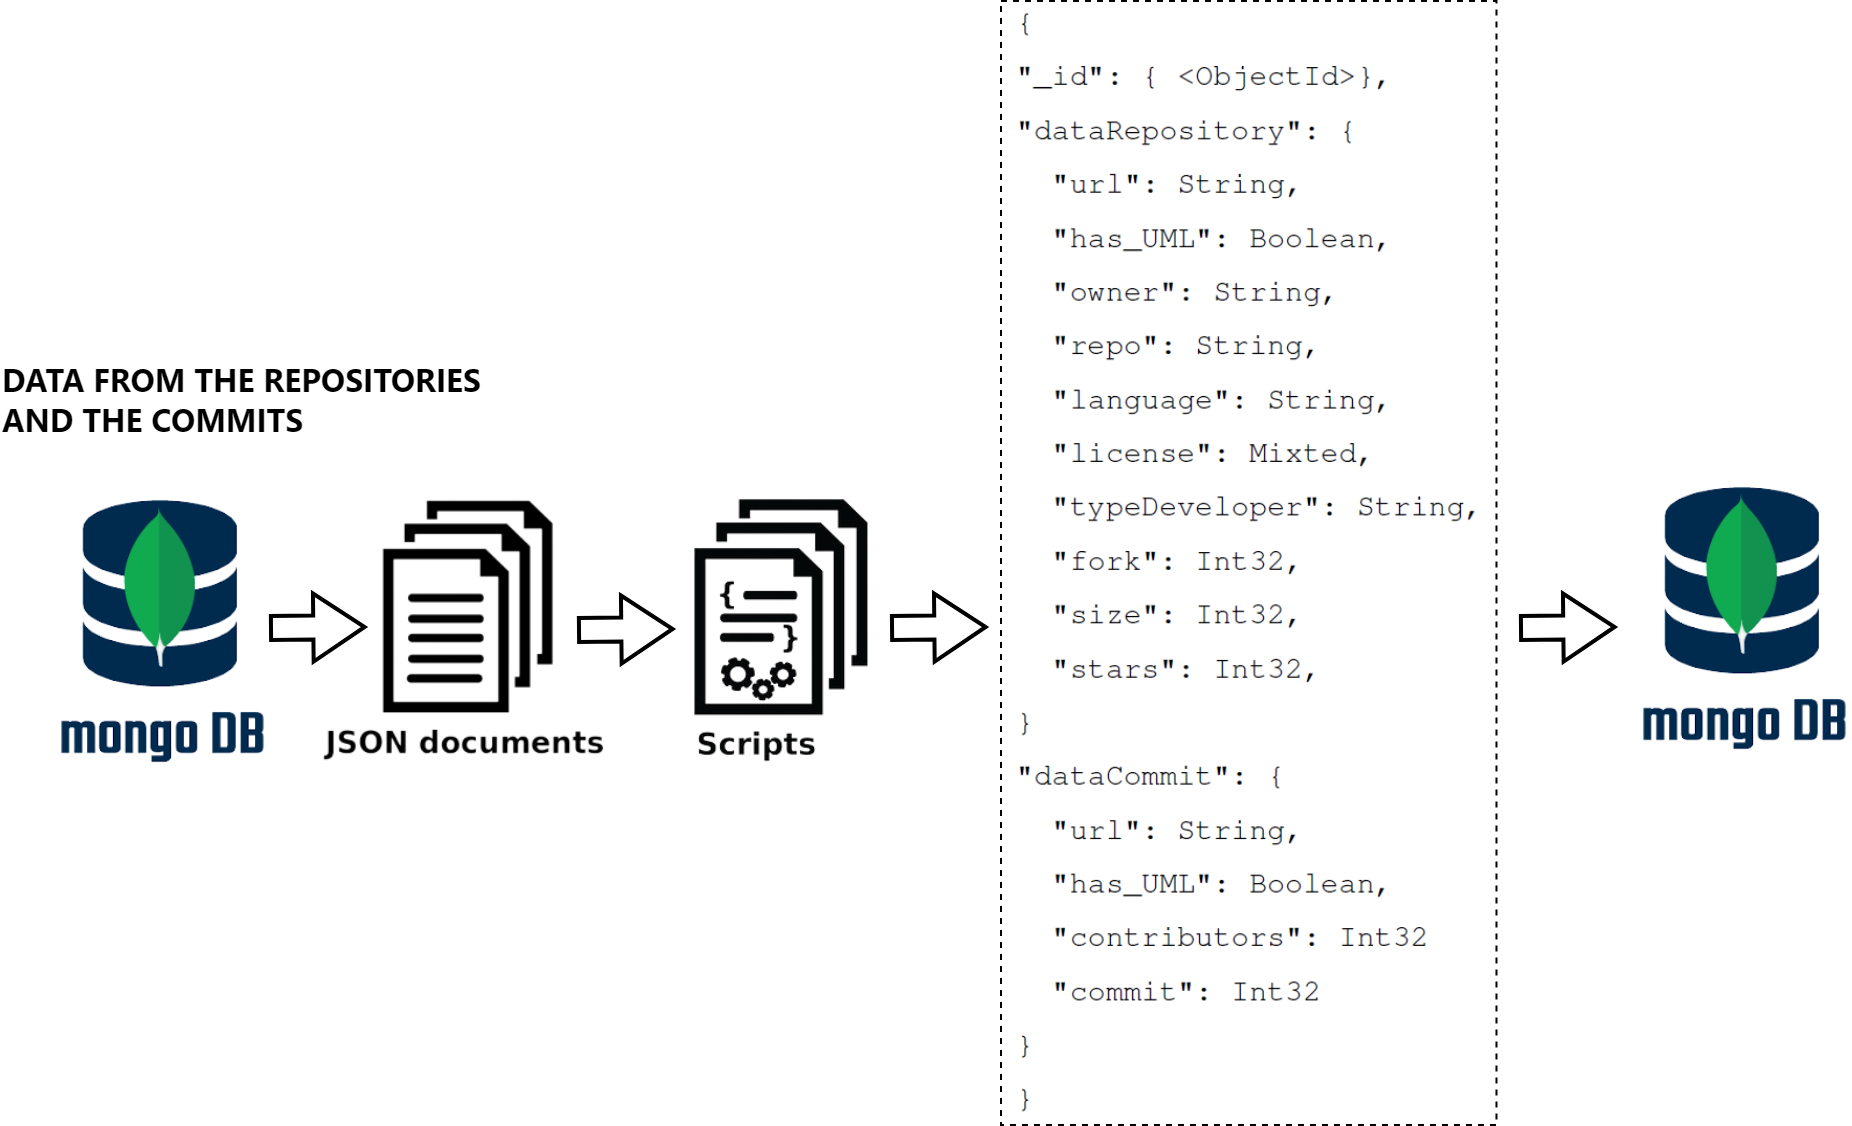
\includegraphics[width=16cm, keepaspectratio]{img/procesamiento_datos.png}
  \caption{Descripción de la fase de procesamiento de datos.}\label{fig:procesamiento_datos}
\end{figure}

Para almacenar estos datos se crearon dos ficheros que se conectan a MongoDB y, a partir de aquí, se crea en cada uno de ellos una nueva coleción con la que se introducen los datos que le pasamos.
A la hora de importar los datos se decidió usar una estructura de diccionario para almacenar los datos extraídos de los repositorios y otra para almacenar los datos de los commits de dichos repositorios.
La siguiente estructura diccionario ha sido usada para guardar la información que se utilizará en el posterior análisis. 


Esta estructura se utilizó para guardar los datos obtenidos de los repositorios y de los commits realizados en los mismos:
{\footnotesize
\begin{verbatim}
  {
  "_id": { <ObjectId>},
  "dataRepository": {
    "url": String,
    "has_UML": Boolean,
    "owner": String,
    "repo": String,
    "language": String,
    "license": Mixted,
    "typeDeveloper": String,
    "fork": Int32,
    "size": Int32,
    "stars": Int32,
  }
  "dataCommit": {
    "url": String,
    "has_UML": Boolean,
    "contributors": Int32
    "commit": Int32
  }
  }
\end{verbatim}
}


A continuación, se explicarán los datos extraídos de los repositorios y los commits que se han guardado en esta estructura:
\begin{itemize}

  \item ``url'': se refiere a la ubicación del repositorio.
  Esta información se usa cuando un usuario quiere clonar un repositorio de GitHub.

  \item ``has\_UML'': en este campo se indica si en dicho repositorio se usan archivos UML o no.
  Dado que este campo es un Boolean, los valores de este campo pueden ser ``True'', si en el proyecto existen diagramas de este tipo, o ``False'', si en el proyecto no existen diagramas UML.
  
  \item ``owners'': en este campo se muestra el nombre del propietario del repositorio. 
  Es decir, el usuario o la organización que creó el repositorio y que es responsable de los cambios que se producen en él. 
  Con este campo se puede acceder a otros repositorios que sean propiedad del mismo usuario u organización. 
  Además, también, se puede utilizar para identificar el perfil de GitHub del propietario del repositorio y ponerse en contacto con él.

  \item ``repo'': nos muestra el nombre del repositorio, este es un identificador que se utiliza para acceder al repositorio, es decir, incluye tanto el nombre del usuario u organización, como el nombre del repositorio en sí, separados por una barra diagonal (/).
  Esta información nos sirve para identificar el repositorio al que pertenece la información extraída.

  \item ``language'': nos muestra el lenguaje de programación principal utilizado en el repositorio.
  Los valores que se encuentran en este campo pueden ser, por ejemplo, ``Python'', ``Java'', ``JavaScript'', ``C++'', ``Ruby'', entre otros.
  
  \item ``license'': en este campo se muestra la licencia bajo la cual está disponible el código fuente del proyecto.
  Para que un repositorio sea verdaderamente de código abierto, ha de tener una licencia. 
  Con esta licencia cada propietario define el marco legal en el que se puede usar, distribuir o modificar el proyecto.
  Algunas licencias pueden ser más restrictivas que otras en cuanto a los derechos que otorgan a los usuarios y desarrolladores de software.
  
  \item ``typeDeveloper'': se indica si el repositorio en cuestión pertenece a un usuario individual o a una organización. 
  Los valores pueden ser ``User'', si el propietario del repositorio es un usuario individual u ``Organization'', si el propietario del repositorio es una organización y no un usuario individual. 
  Las organizaciones en GitHub están formadas por grupos de personas que trabajan juntas en un proyecto o en varios proyectos relacionados.
  
  \item ``fork'': se indica si ese repositorio es una copia de otro repositorio existente en GitHub. 
  Los valores de este campo pueden ser ``true'', que significa que el repositorio es una bifurcación o ``fork'' de otro repositorio en GitHub o ``false'', que significa que el repositorio no es una copia de ningún otro repositorio de GitHub.
  Los usuarios de GitHub utilizan los ``fork'' para crear nuevas versiones de un proyecto existente para agregar nuevas funcionalidades, corregir errores, o personalizar un proyecto original.
  Cada vez que se crea un ``fork'', se crea una copia completa del repositorio original en el que se pueden realizar cambios sin afectar al repositorio original.
  
  \item ``size'': este dato se refiere al tamaño de almacenamiento que ocupa el repositorio en kilobytes, megabytes o gigabytes.  
  Al conocer el tamaño de un repositorio nos hacemos una idea de la magnitud del proyecto.

  \item ``stars'': señala el número de usuarios que han marcado el repositorio como favorito, ya sea porque el repositorio le resulta interesante o útil al usuario.
  Esta información nos muestra qué repositorios son más relevantes o valorados por la comunidad de GitHub dependiendo de la cantidad de ``stars'' que tengan.

  \item ``contributors'': nos indica el número de personas que han participado en el repositoio al haber realizado commits en los cuales se ha contribuido a la mejora del proyecto del propietario del repositorio.
  Un gran número de colaboradores nos indica que el desarrollo del proyecto del repositorio es mayor frente a uno con pocos colaboradores.
  
  \item ``commit'': se muestra el número de commits qua se han realizado en el repositorio.
  Un ``commit'' es una acción que se realiza para guardar los cambios realizados en los archivos de un repositorio.
  Todos estos ``commits'' forman el historial del repositorio y permiten a los usuarios tener la posibilidad de revisar las modificaciones realizadas y revertir cambios en caso de ser necesario. 
  Por lo tanto, el número de commits nos puede indicar el nivel de actividad de un proyecto, así como la frecuencia de actualizaciones, mejoras y mantenimiento del mismo.
 
\end{itemize} 

\section{Análisis de datos} % título de sección (se muestra)
\label{sec:análisis de datos}

Con el análisis de datos, que es el objetivo final del proyecto, se pretende conocer las similitudes y diferencias entre los desarrolladores que utilizan archivos UML y el resto de los desarrolladores que no utilizan este tipo de archivos.


En esta sección se describe el proceso de análisis de los datos obtenidos, a partir de Perceval, de los distintos repositorios de GitHub. 
Se comenzó por la revisión y limpieza de los datos, eliminando aquellos que decidimos no incluir, ya que no se consideraban datos relevantes para el análisis que pretendemos hacer. 
A partir de aquí, se procedió a la exploración de los datos, mediante el cálculo de estadísticos descriptivos, para cada una de las variables de interés. 
Para ello se realizó un fichero en el que se ejecuta el análisis de los datos extraídos usando Python, observando así las diferencias entre los desarrolladores que utilizan UML y el resto.
A este fichero se le pasaron los 400 datos recogidos; de los cuales, la mitad son repositorios que usan archivos UML y la otra mitad repositorios que no usan archivo UML. 
En el fichero desarrollado se han analizado los siguientes datos de cada uno de los repositorios. 


En primer lugar, se comentarán los datos que se han usado en el análisis de cada uno de los repositorios y el cálculo estadístico que se ha llevado a cabo en cada uno de ellos:


\subsection{Lenguaje de programación principal del repositorio} % título de subsección (se muestra)
\label{sec:lenguaje de programación principal del repositorio}
Para comprobar los lenguajes de programación que tienen mayor presencia, en los repositorios con y sin diagramas UML, se han recogido los nombres de todos los lenguajes de programación que predominan en los documentos JSON generados.
Con esta información se realizará la media de estos datos siguiendo la siguiente fórmula para cada uno de los diez lenguajes de programación que se han seleccionado.


\[{Lenguaje X} = \frac{1}{400} \sum_{i=1}^{400} x_i\]


\subsection{Licencia del repositorio} % título de subsección (se muestra)
\label{sec:licencia del repositorio}
También nos interesa conocer el número de repositorios que tienen licencia y cuáles no.
Para ello se realiza un proceso de análisis estadístico de los repositorios para saber si tienen o no licencia.
Para cada repositorio, se ha accedido al valor ``Licencia'' de los documentos JSON obtenidos con Perceval y se ha registrado la información correspondiente.

En este análisis lo primero será extraer cada uno de los documentos JSON, que hemos generado, para guardar los puntos a analizar de cada desarrollador.
De cada uno de estos documentos se obtendrán los valores almacenados en el campo ``Licencia''.
Posteriormente, se comprobará si el objeto JSON tiene información en el valor ``Licencia''; si el valor es nulo, se entiende que el repositorio no tiene licencia.


\begin{equation}
  Licencia =
  \begin{cases}
  [licencia], & \text{si el repositorio tiene una licencia} \\
  null, & \text{si el repositorio no tiene una licencia}
  \end{cases}
\end{equation}

Después de recoger los resultados de esta función comparativa, se procede a realizar la media de todos repositorios con y sin archivos UML.
\[{Licencia} = \frac{1}{400} \sum_{i=1}^{400} x_i\]


\subsection{Tipo de propietario del repositorio} % título de subsección (se muestra)
\label{sec:tipo de propietario del repositorio}

Otro de los datos relevantes que nos interesa saber es el tipo de propietario de los repositorios, si usuario individual o bien un usuario que es una organización. 
Para ello se procede a estudiar el promedio de los tipos de propietarios de los desarrolladores UML y del resto de los desarrolladores.
Los posibles tipos de propietarios que puede haber son ``User'', si es un usuario individual o bien un usuario que es una ``Organization'' si se trata de una organización compuesta por varios usuarios.
Esta información se muestra también en los documentos JSON obtenidos de los repositorios.

\begin{equation}
  Propietario =
  \begin{cases}
  User, & \text{si el propietario del repositorio es un usuario individual} \\
  Organization, & \text{si el propietario del repositorio es una organización}
  \end{cases}
\end{equation}

Después de haber definido los propietarios de cada uno de los repositorios, se realizará la media de todos ellos para conocer si los repositorios que contienen archivos UML suelen ser propiedad de organizaciones o de usuarios individuales.
A continuación se muestra la fórmula usada para realizar las medias de los repositorios cuyos propietarios son usuario o desarrolladores:

\[{User} = \frac{1}{400} \sum_{i=1}^{400} x_i\]
\[{Organization} = \frac{1}{400} \sum_{i=1}^{400} x_i\]


\subsection{Número de fork por repositorio} % título de subsección (se muestra)
\label{sec:Número de fork por repositorio}

Otro de los datos que nos interesa en este análisis es conocer si se han hecho bifurcaciones de los respositorios.
En los datos extraídos de los repositorios con Perceval se encuentra el campo ``forks'', con el cual se comprueba el número de bifurcaciones (``forks'') del repositorio.
En caso de que el valor de este campo sea distinto de ``0'' , se habrán realizado ``forks''; en caso contrario, no se habrán realizado ``forks'' en el repositorio.


Una vez que se han definido el número de ``forks'' de cada repositorio, se procederá a realizar la media de todos ellos para conocer el número de ``forks'' medio que se suele realizar en los repositorios con UML con respecto al resto de repositorios si diagramas UML.
A continuación se muestra la fórmula usada para realizar la media del número de ``forks'' por repositorio:


\[{Fork} = \frac{1}{400} \sum_{i=1}^{400} x_i\]


\subsection{Número de stars por repositorio} % título de subsección (se muestra)
\label{sec:número de stars por repositorio}

Otro dato significativo, que nos interesa de los extraídos en los repositorios, es el número de ``stars'' por repositorio.
Este número nos muestra la cantidad de usuarios que han marcado dicho repositorio como favorito y, por tanto, nos indica la popularidad de éste dentro de la comunidad. 
Para obtener el número de ``stars'' por repositorio buscaremos el campo ``stargazers count'' en los datos extraídos mediante Perceval. 
Después de realizar una recopilación con el número de ``stars'' por repositorio, se realizará la media entre todos los repositorios.

\[{Stars} = \frac{1}{400} \sum_{i=1}^{400} x_i\]


\subsection{Tamaño del repositorio} % título de subsección (se muestra)
\label{sec:tamaño del repositorio}
Este dato informa sobre el tamaño aproximado de un repositorio en kilobytes. 
Para ello, utilizaremos dos diagramas de caja para analizar y contrastar el tamaño de los repositorios, lo que nos permitirá obtener información descriptiva más completa, tanto de la distribución de los tamaños de los repositorios con diagramas UML. como de la distribución de los tamaños de los repositorios sin utilizar dichos diagramas.


Un diagrama de caja~\cite{neto2017boxplot} es una representación gráfica que muestra la distribución de un conjunto de datos.
En esta representación gráfica se pueden observar de manera visual varios valores estadísticos, como podemos ver en la figura ~\ref{fig:boxplot}.
Estos valores estadísticos que podemos encontrar en un diagrama de caja son: el rango intercuartílico (RIC) que se representa como una caja rectangular y es el rango que abarca el 50\% de los datos, la línea dentro de la caja representa la mediana, 
los bigotes que se encuentran en los extremos de la caja, los cuales representan los valores máximo y mínimo de los valores de nuestra distribución de datos y, por último, los valores atípicos que se representan mediante puntos colocados por encima del bigote superior o por debajo del bigote inferior.
Dichos valores atípicos representan valores inusuales dentro de la distribución de datos.


Todos estos valores estadísticos nos ayudarán a entender mejor la distribución del tamaño total por repositorio, puesto que se mostrará la media del tamaño por repositorio, la variabilidad que hay en los distintos repositorios, etc.

\begin{figure}
  \centering
  
\includegraphics[width=8cm, keepaspectratio]{img/Boxplot.png}
  \caption{Representación de un diagrama de caja.}\label{fig:boxplot}
\end{figure}

A continuación, se comentarán los datos utilizados en el análisis obtenidos a partir de los commits de los repositorios y los cálculos empleados en cada caso.
Para analizar los datos extraídos de los commits calcularemos los diagramas de caja para obtener una información visual más descriptiva de cada una de las distribuciones de datos.


\subsection{Número de colaboradores por repositorio} % título de subsección (se muestra)
\label{sec:número de colaboradores por repositorio}

En este caso se va a realizar un diagrama de caja con el conjunto de datos sobre el número de personas que hacen commits por repositorio.
El número de personas que han realizado commits en un repositorio nos indica si hay una colaboración grande o pequeña en el desarrollo del repositorio.
Este dato a analizar se obtiene de los documentos JSON extraídos de los commits realizados en cada repositorio, por lo que se realizarán dos diagramas de caja.
Uno de ellos nos dará una representación visual de la distribución del conjunto del número de colaboradores en repositorios con diagramas UML y el otro nos dará una representación visual de la distribución del conjunto del número de colaboradores en repositorios sin diagramas UML.
Con este tipo de representación se puede observar varios valores estadísticos del conjunto de datos, como se ha mencionado anteriormente.


Nos fijaremos en la variabilidad de los datos. Para ello, se observarán los cuartiles que dividen un conjunto de datos ordenados en cuatro partes iguales.
El valor del primer cuartil (Q1) divide el conjunto de los datos en el 25\% que contienen los datos más bajos de dicho conjunto; la mediana que divide el conjunto de datos en el 50\% y el tercer cuartil (Q3) que representa el 25\% de los datos con valores más altos.
Además de observar estos datos, examinaremos el rango en el que se concentran los datos que se corresponde con el rango intercuartílico (RIC) y se calcula mediante la diferencia entre el tercer cuartil y el primer cuartil (RIC = Q3 - Q1).


Por último, nos fijaremos en los valores atípicos, esto es, en el conjunto de datos que indican valores inusuales.
Estos valores se calculan siguiendo las siguientes fórmulas que nos dan los valores atípico inferiores al primer cuartil (Q1 - RIC * 1.5)  o los valores superiores al tercer cuartil (Q3 + RIC * 1.5). 


% Todos estos valores estadísticos nos ayudarán a entender mejor la distribución del número de colaboradores por repositoio, puesto que se mostrará la media de colaboradores por repositoio y la variabilidad que hay en el número de colaboradores.

\subsection{Cantidad total de commits por repositorio} % título de subsección (se muestra)
\label{sec:cantidad total de commits por repositorio}

En este capítulo, acabaremos analizando el número total de commits que se han realizado en cada uno de los repositorios.
Este dato representa la cantidad de cambios o actualizaciones que se han llevado a cabo en el código del proyecto.
Lo que nos puede dar una idea de si se ha dedicado una gran cantidad de tiempo en un proyecto o no y, por tanto, esto nos dice si el proyecto en sí es grande o no lo es. 


Para examinar el conjunto de datos del número de commits, que se realizan en los repositorios que usan archivos UML y los que no los usan, se usará la representación de  los diagramas de caja como se ha hecho en el caso anterior.
Realizaremos esta representación a partir del conjunto de datos relacionados con el número total de commits de cada repositorio que se encuentran almacenados en los documentos JSON de la base de datos de MongoDB.
Estos documentos JSON los analizaremos separando los repositorios con UML del resto de repositorios. 
Por tanto, se realizarán dos diagramas de caja con una distribución de 200 datos en cada una de ellas, para comparar la distribución del número de commits que se ha realizado en los repositorios con diagramas UML y la distribución del número de commits que se han realizado en repositorios sin diagramas UML.
Con estos diagramas de caja se observarán los distintos valores estádísticos, mencionados anteriormente, para tener una información visual de ambas distribuciones de datos y analizar las diferencias entre éstas.  


%%%%%%%%%%%%%%%%%%%%%%%%%%%%%%%%%%%%%%%%%%%%%%%%%%%%%%%%%%%%%%%%%%%%%%%%%%%%%%%%
%%%%%%%%%%%%%%%%%%%%%%%%%%%%%%%%%%%%%%%%%%%%%%%%%%%%%%%%%%%%%%%%%%%%%%%%%%%%%%%%
% RESULTADOS %
%%%%%%%%%%%%%%%%%%%%%%%%%%%%%%%%%%%%%%%%%%%%%%%%%%%%%%%%%%%%%%%%%%%%%%%%%%%%%%%%

\cleardoublepage
\chapter{Resultados}
\label{chap:resultados}

 
En este capítulo se presentan los resultados obtenidos a partir del análisis de los datos recopilados de 200 repositorios de GitHub con archivos UML y 200 repositorios sin dichos archivos.
Recordemos que el objetivo de este análisis es comparar estos tipos de repositorios para ver las similitudes y diferencias que existen entre ellos.
Para ello se ha realizado una recolección de datos y un análisis estadístico para establecer patrones en los repositorios con archivos UML y en los que no hay archivos UML.


\section{Descripción de los datos recopilados}
\label{sec:descripción de los datos recopilado}

Los datos recopilados para el análisis de este proyecto se obtuvieron de una selección de repositorios públicos almacenados en GitHub. 
Estos repositorios pueden contener archivos de código, documentación y otros tipos de archivos, como los  ``.uml''.
Estos archivos ``.uml'' junto con otros formatos de archivos, como los ``.png'', ``.jpg'',``.xmi'' , entre otros, pueden almacenar diagramas UML y, por tanto, estos serán los archivos que dividan los datos obtenidos para el análisis de nuestro estudio en los repositorios que los contengan y en los que no.


Para la selección de los 400 repositorios que se han analizado en este proyecto, se han escogido 200 repositorios que contienen diagramas UML, los cuales han sido obtenidos de la base de datos Lindholmen dataset\footnote{\url{http://models-db.com/}}, que contiene una lista con los repositorios que utilizan diagramas UML en GitHub.


En cuanto a los repositorios que no tienen diagramas UML, estos se han recopilado manualmente de los usuarios que siguen o son colaboradores de los usuarios que aparecen en la lista de los repositorios con diagramas UML.


Para reunir los datos que se usarán en el análisis del proyecto, se ha recurrido a la herramienta de Perceval, con la cual se han obtenido 400 archivos en formato JSON con todos los datos de cada repositorio de GitHub y otros 400 archivos JSON con los commits generados en estos repositorios.
Estos archivos JSON contienen datos estructurados de toda la información de los repositorios a analizar, lo que nos permitirá organizar y almacenar los datos de interés de cada uno de estos archivos fácilmente. 


Como se ha mencionado anteriormente, el conjunto de los 400 archivos JSON, tanto de los repositorios como de los commits, se ha dividido en aquellos repositorios que contienen diagramas UML y aquellos que no. 
Con esta división de los datos contenidos en los archivos JSON, se analizarán mejor las similitudes y diferencias entre estos repositorios. 


De las características que se pueden observar en cada uno de los archivos JSON, obtenidos tanto de los repositorios como de los commits realizados en estos, se han decidido estudiar las siguientes:
la licencia que determina si el repositorio garantiza derechos y responsabilidades, el tipo de propietario que nos informa sobre si el propietario del repositorio es un usuario individual o una entidad que representa un grupo de personas, 
el número de forks que nos muestra cuántas copias se han realizado del repositorio, el lenguaje de programación predominante que se emplea en el repositorio, el número de stars que nos informa de la cantidad de usuarios que han marcado como favorito el repositorio, 
el tamaño del repositorio, el número de colaboradores que nos proporciona información sobre la cantidad de desarrolladores que realizan commits en el repositorio y la cantidad total de commits que refleja el nivel de actividad de un proyecto.
Para extraer dichas características de los archivos JSON, se ha realizado un procesamiento de los datos que se encuentran en estos archivos.
Con el objetivo de obtener los datos de estas características se han desarrollado varios ficheros de Python con los cuales se sacan los datos que se encuentran en diferentes campos de los archivos JSON.


\section{Interpretación de los resultados del análisis}
\label{sec:interpretación de los resultados del análisis}

Después de recopilar y preprocesar los datos seleccionados se realiza el análisis estadístico de estos.
A partir de aquí, se podrán observar las similitudes y diferencias de los repositorios que se han seleccionado en este estudio.
Una vez obtenidos los resultados del análisis realizado se va llevar a cabo una interpretación de los mismos.


A continuación, se muestran una serie de gráficas que se corresponden con los resultados obtenidos en el análisis de los datos extraídos de los repositorios de GitHub.

\subsection{Principales lenguajes de programación por repositorio}
\label{sec:Gráfico de barras de los lenguages principales de programación por repositorio}

% --------------------------------      LANGUAGES      --------------------------
En este caso vamos a utilizar un gráfico de barras que nos proporciona una visualización clara de la distribución de los lenguajes de programación en los repositorios, permitiéndonos identificar los lenguajes más utilizados.
La siguiente figura ~\ref{fig:Figure_language}, representa la distribución de los lenguajes de programación que predominan en cada uno de los repositorios analizados.
En este gráfico se observa que el lenguaje de programación más utilizado en los repositorios con diagrmas UML es Java, seguido de JavaScript y C++.
En cambio, en los repositorios sin diagramas UML el lenguaje de programación más utilizado es JavaScript, seguido de Python y Java.
Por tanto, los lenguajes de programación más utilizados en los repositorios con diagramas UML y sin estos son JavaScript y Java. 
Esto indica que existe una preferencia generalizada por los lenguaje de Java y JavaScript en la comunidad de desarrollo de los repositorios estudiados.
También se puede observar que en los repositorios con diagramas UML hay un elevado porcentaje de estos que tienen como lenguaje principal de programación otros lenguajes distintos a los evaluados en este estudio.


Por otro lado, el lenguaje de C++ tiene aproximadamante la misma presencia en repositorios con y con diagramas UML, aunque en menor medida en comparación con JavaScript o Java.
Esto sugiere que este lenguaje también es bastante utilizado, pero no alcanza el mismo nivel de popularidad.
Por último, mencionar que en los repositorios con UML que hemos usado en este estudio en ninguno de ellos predominan los lenguajes de programación TypeScript y Swift.

\begin{figure}
  \centering
  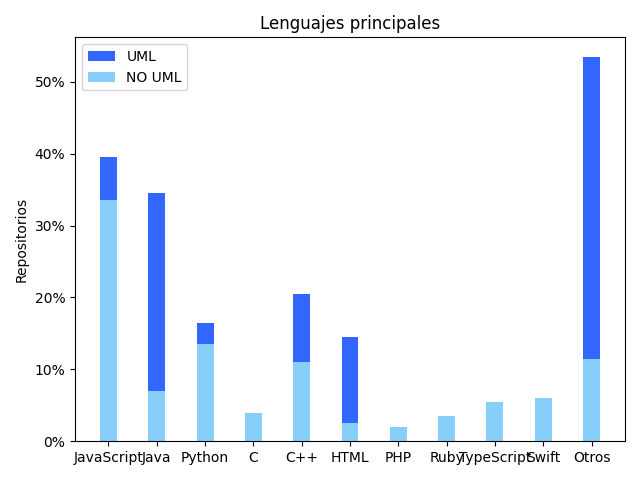
\includegraphics[width=12cm, keepaspectratio]{img/Figure_languages.png}
  \caption{Porcentaje de repositorios por lenguaje principal de programación.}\label{fig:Figure_language}
\end{figure}

\subsection{Repositorios con licencia y sin licencia}
\label{sec:Gráfico de barras de los repositorios con licencia y sin licencia}

% --------------------------------      LICENSE      --------------------------
Para visualizar el porcentaje de repositorios con licencia y sin licencia también se ha utilizado un gráfico de barras.
En la figura ~\ref{fig:Figure_license} se observa que el casi el 40\% de los repositorios con diagramas UML tienen licencia, mientras que en los repositorios sin diagramas UML cerca del 20\% aproximadamante tienen licencia.
Esto indica que los repositorios con diagramas UML tienen una tendencia significativamente mayor a contar con una licencia en comparación con aquellos que no contienen dichos diagramas.

\begin{figure}
  \centering
  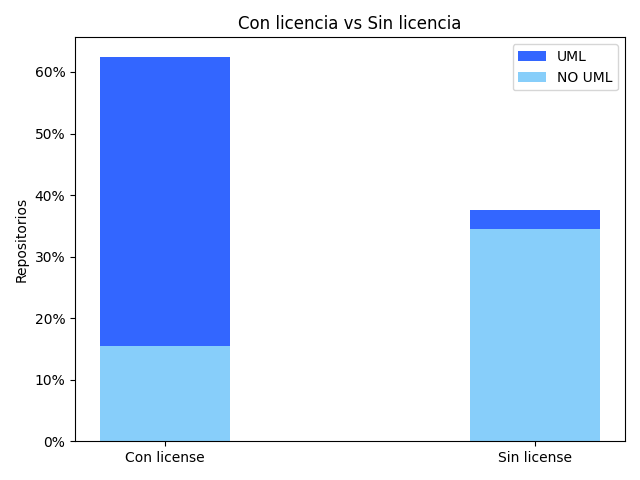
\includegraphics[width=12cm, keepaspectratio]{img/Figure_license.png}
  \caption{Porcentaje de repositorios con licencia y sin licencia.}\label{fig:Figure_license}
\end{figure}

\subsection{Propietarios de los repositorios que son usuarios individuales y organizaciones}
\label{sec:Gráfico de barras de los propietarios de los repositorios que son usuarios individuales y organizaciones}
% ------------------------------    TYPE DEVELOPER     --------------------------------------------

En la figura ~\ref{fig:Figure_typeDeveloper} se presenta un gráfico de barras que muestra el porcentaje de propietarios de los repositorios, distinguiendo entre usuarios individuales y organizaciones. 
Los resultados revelan que en los repositorios con y sin diagramas UML alrededor de un 40\% son propiedad de usuarios individuales, mientras que en torno al 10\% son propiedad de organizaciones.
Estos resultados señalan que en ambos tipos de repositorios hay una tendencia similar a que los propietarios sean usuarios individuales.


\begin{figure}
  \centering
  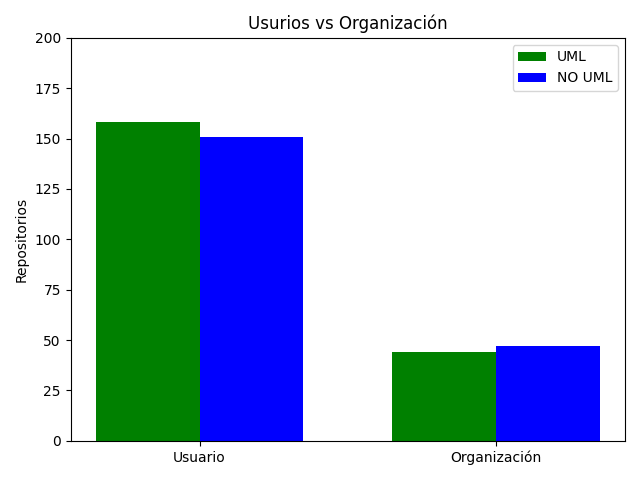
\includegraphics[width=12cm, keepaspectratio]{img/Figure_typeDeveloper.png}
  \caption{Porcentaje de propietarios que son ususarios individuales y organizaciones.}\label{fig:Figure_typeDeveloper}
\end{figure}


\subsection{Repositorios con fork y sin fork}
\label{sec:Gráfico de barras de los repositorios con fork y sin forks}
% --------------------------------      FORKS      --------------------------
En la siguiente figura ~\ref{fig:Figure_fork} se observa un gráfico de barras con los porcentajes de  los repositorios con y sin diagramas UML que tienen o no tienen forks.
Los resultados obtenidos muestran una notable disferencia entre los repositorios que contienen diagramas UML y los que no los contienen.
En particular, se destaca que aproximadamante el 40\% de los repositorios con diagramas UML no tienen fork, en cambio cerca del 40\% de los repositorios sin diagramas UML si tienen fork.
Estos resultados reflejan que los repositorios con diagramas UML tienen una tendencia significativamente mayor a que se realicen forks en dichos repositorios.

\begin{figure}
  \centering
  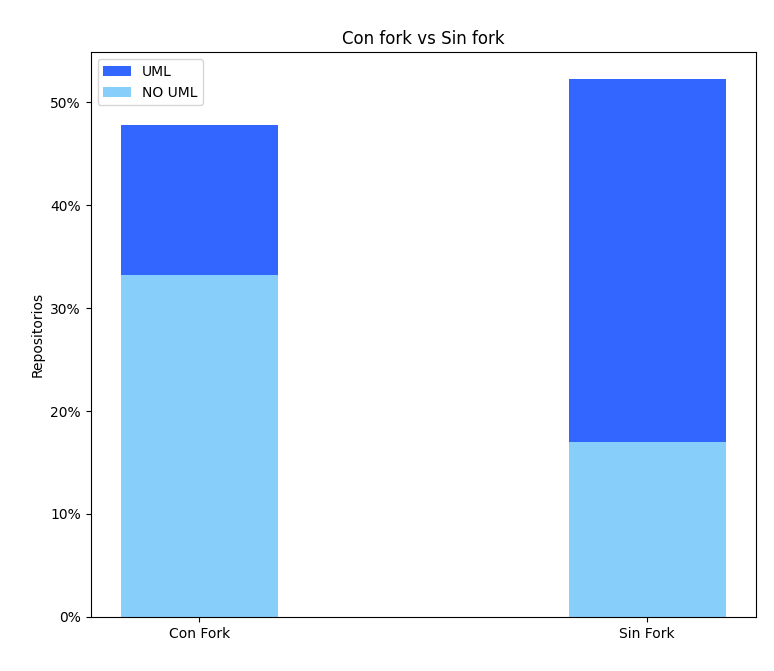
\includegraphics[width=12cm, keepaspectratio]{img/Figure_fork.png}
  \caption{Porcentaje de repositorios con fork y sin fork.}\label{fig:Figure_fork}
\end{figure}


\subsection{Stars por repositorio}
\label{sec:Gráfico de barras de los stars por repositorio}
% --------------------------------      STARS     --------------------------
En esta figura ~\ref{fig:Figure_stars} también se utiliza un gráfico para ofrecer información visual acerca de la distribución de los repositorios que tienen stars. 
Comparando los resultados obtenidos se puede observar que hay una diferencia significativa entre los repositorios con diagramas UML y los que no los contienen.
Se muestra claramente que el 40\% de los repositorios con diagramas UML tienen stars, mientras que en los repositorios sin diagramas UML solo cerca del 20\% tienen stars.
Estos datos indican de manera clara que los repositorios con diagramas UML no son tan populares como los que no los contienen.

\begin{figure}
  \centering
  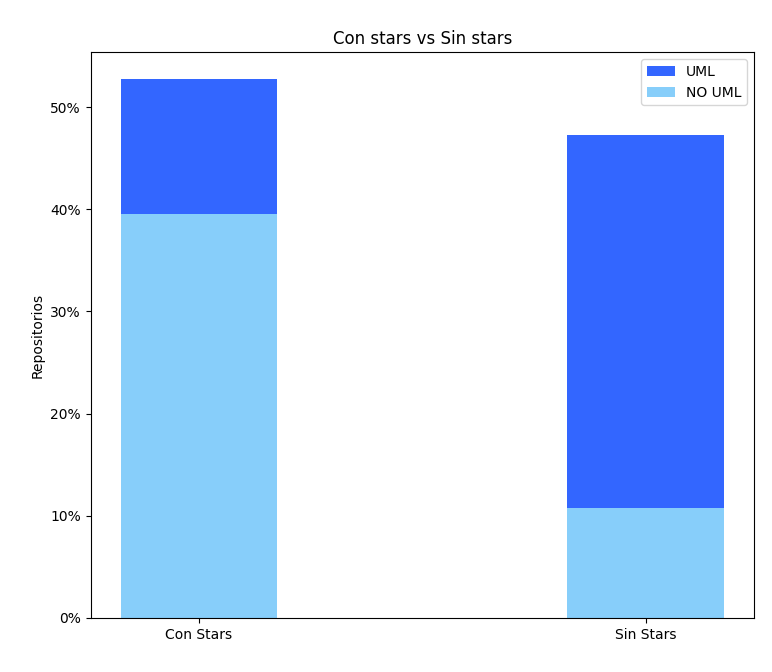
\includegraphics[width=12cm, keepaspectratio]{img/Figure_stars.png}
  \caption{Porcentaje de stars por repositorio.}\label{fig:Figure_stars}
\end{figure}


\subsection{Tamaño de los repositorios}
\label{sec:Diagrama de caja del tamaño de los repositorios}
% ------------------------------      SIZE      ----------------------------
En la figura ~\ref{fig:Figure_sizeUML} se representa una visualización de diagrama de caja que muestra la distribución de los tamaños de los repositorios que tienen diagramas UML 
mientras que en la figura ~\ref{fig:Figure_sizeNOUML} se representa el tamaño de los repositorios que no tienen diagramas UML.
Se realizará una comparación de ambos diagramas de caja para comprender las difencias de las distribuciones de datos del tamaño de los repositorios que contiene diagramas UML y que los contienen.
 

En cuanto al rango intercuartílico, en la figura ~\ref{fig:Figure_sizeUML} observamos que es claramente mayor en comparación con el rango intercuartílico de la figura ~\ref{fig:Figure_sizeNOUML}.
Esto se debe a que los repositorios que contienen diagramas UML tienen un tamaño mayor que los repositorios que no los contienen y por tanto el rango intercuartílico es mayor.
En la figura ~\ref{fig:Figure_sizeUML} este rango llega en torno a los 4000 KB, mientras que en la figura ~\ref{fig:Figure_sizeNOUML} el rango intercuartílico llega hasta los 2000 KB.


Al comparar la mediana que se corresponde con la línea roja, que se encuentra en el interior de ambos diagramas de caja, se observa que la mediana de la figura ~\ref{fig:Figure_sizeUML} es ligeramente mayor que la mediana de la figura ~\ref{fig:Figure_sizeNOUML}.
Esta mediana se encuentra en torno a los 500 KB en ambas figuras.


Comparando el valor máximo en cada figura, nos damos cuenta de que en la figura ~\ref{fig:Figure_sizeUML} el valor máximo es mayor y se encuentra en los 6000 KB aproximadamante, mientras que en la figura ~\ref{fig:Figure_sizeNOUML} el valor máximo está cerca de los 4000 KB.
En cuanto a los valores atípicos, en ambas figuras hay una gran cantidad de ellos debido a que en los repositorios de nuestro estudio hay una gran cantidad de valores atípicos que tienen un tamaño más elevado que el del resto de la distribución.

\begin{figure}
  \centering
  \begin{subfigure}{0.45\linewidth}
    \centering
    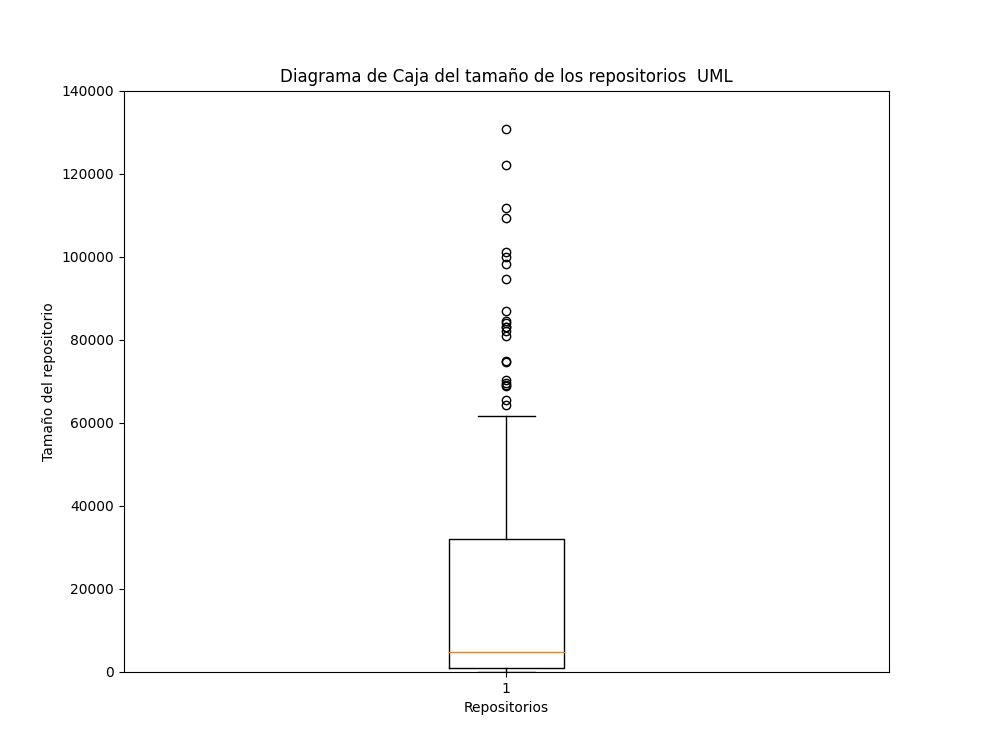
\includegraphics[width=9cm, keepaspectratio]{img/Figure_sizeUML.png}
    \caption{Diagrama de caja del tamaño total por repositorio con diagrama UML.}\label{fig:Figure_sizeUML}
  \end{subfigure}
  \hfill
    \begin{subfigure}{0.45\linewidth}
      \centering
      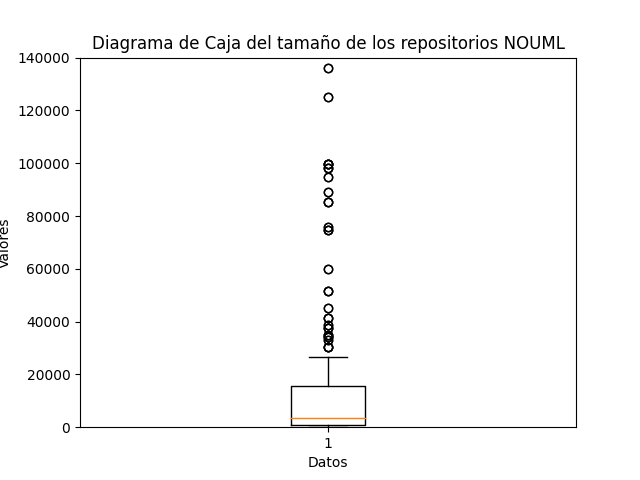
\includegraphics[width=9cm, keepaspectratio]{img/Figure_sizeNOUML.png}
      \caption{Diagrama de caja del tamaño total por repositorio sin diagrama UML.}\label{fig:Figure_sizeNOUML}
  \end{subfigure}
\end{figure}

\subsection{Colaboradores por repositorio}
\label{sec:Diagrama de caja de los colaboradores por repositorio}
% --------------------------------      CONTRIBUTORS     --------------------------
En la figura ~\ref{fig:Figure_contributorsUML} se muestra el diagrama de caja que refleja la distribución del número de forks de los repositorios con diagramas UML mientras que en la figura ~\ref{fig:Figure_contributorsNOUML} el diagrama de caja se corresponde con aquellos repositorios sin diagramas UML.


En este caso comparando las figuras ~\ref{fig:Figure_contributorsUML} y ~\ref{fig:Figure_contributorsNOUML} se observa una gran diferencia en el rango intercuartílico (RIC) de cada una de ellas.
La figura ~\ref{fig:Figure_contributorsUML} tiene un rango muy pequeño de número de colaboradores, la mayoría de repositorios con diagramas UML tienen menos de 10 colaboradores por repositorio.
Sin embargo, en la figura ~\ref{fig:Figure_contributorsNOUML} se aprecia claramente que este rango tiene una mayor dispersión de los datos llegando en torno a 45 colaboradores en algunos repositorios. 
Esto quiere decir que en los repositorios que no contienen diagramas UML hay una mayor participación de desarrolladores que realizan commits en estos repositorios.


Si comparamos la mediana de ambas figuras representada con la línea roja, también se aprecia una pequeña diferencia entre estas. 
En los repositorios con diagramas UML la mediana se encuentra en 5 colaboradores aproximadamente por repositorio, en cambio, en los repositorios sin diagramas UML la mediana llega casi a los 10 colaboradores por repositorio.


En cuanto a los valores máximos de cada una de las distribuciones, vemos que en la figura ~\ref{fig:Figure_contributorsUML} el valor máximo de nuestra distribución se encuentra sobre los 10 colaboradores por repositorio, mientras que en la figura ~\ref{fig:Figure_contributorsNOUML} está aproximadamente en 80 colaboradores por repositorio.


Por último, destacar que ambas figuras tienen varios valores atípicos, en la ~\ref{fig:Figure_contributorsUML} se observa que en la mayoría de estos valores atípicos se concentran al rededor de 20 colaboradores, a diferencia de los valores atípicos de los repositorios sin diagramas UML que se encuentran por encima de los 80 colaboradores por repositorio. 
Estos valores atípicos nos indican que sólo en unos pocos repositorios el número de colaboradores es mayor con respecto al conjunto de la distribución de datos.

\begin{figure}
  \centering
  \begin{subfigure}{0.45\linewidth}
    \centering
    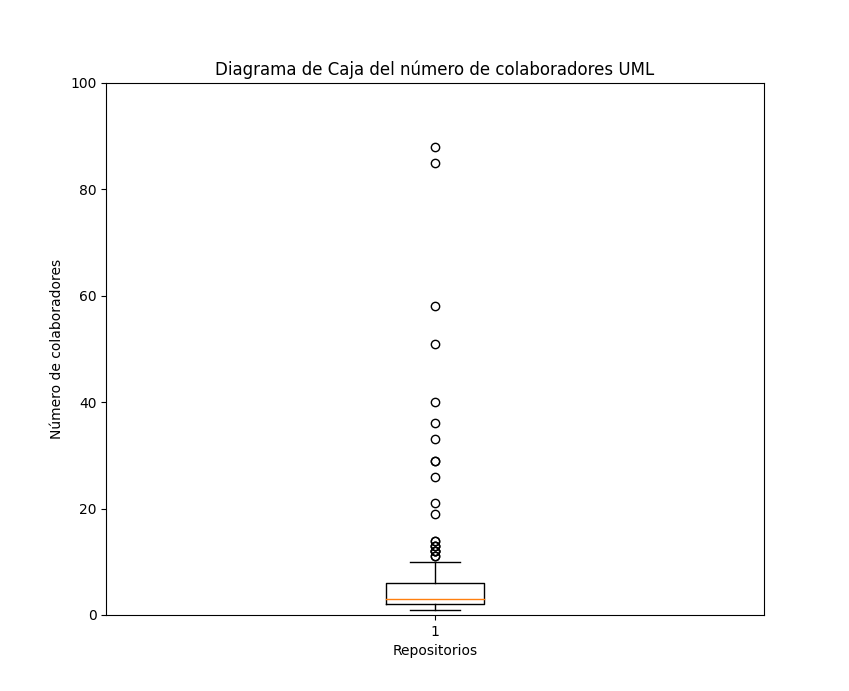
\includegraphics[width=9cm, keepaspectratio]{img/Figure_contributorsUML.png}
    \caption{Diagrama de caja del número de colaboradores total por repositorio con diagrama UML. }\label{fig:Figure_contributorsUML}
  \end{subfigure}
  \hfill
    \begin{subfigure}{0.45\linewidth}
      \centering
      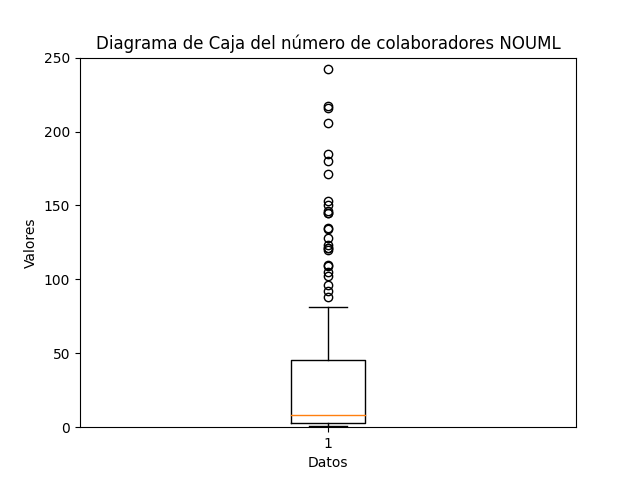
\includegraphics[width=9cm, keepaspectratio]{img/Figure_contributorsNOUML.png}
      \caption{Diagrama de caja del número de colaboradores total por repositorio sin diagrama UML.}\label{fig:Figure_contributorsNOUML}
  \end{subfigure}
\end{figure}

\subsection{Commits por repositorio}
\label{sec:Diagrama de caja de los commits por repositorio}
% --------------------------------      COMMITS        --------------------------
En la figura ~\ref{fig:Figure_commitsUML} y ~\ref{fig:Figure_commitsNOUML} se observan los diagramas de caja que representan la distribución del conjunto de número de commits de los repositorios que tienen y no tienen diagramas UML.


La línea roja en la caja muestra el valor de la mediana; por un lado, vemos que en ambas figuras la mediana se encuentra próxima al primer cuartil, el cual se corresponde con los valores más bajos del conjunto de valores de nuestra distribución. 
Sin embargo, por otro lado, al comparar el diagrama de caja de la figura ~\ref{fig:Figure_commitsUML} con el de la figura ~\ref{fig:Figure_commitsNOUML}, apreciamos que la mediana tiene un valor menor en la figura ~\ref{fig:Figure_commitsUML}, lo que indica que se realizan menos commits de promedio en los repositorios con diagramas UML. 
En otras palabras, hay una concentración de valores más bajos en el conjunto de datos. 
Esto quiere decir que en la mayoría de los repositorios con diagramas UML se realizan menos commits que en los repositorios sin diagramas UML.

 
Observando la longitud de la caja, conocida como rango intercuartílico (RIC), nos damos cuenta de que el número de commits es mayor en el conjunto de los repositorios sin diagramas UML que en el conjunto de los repositorios con diagramas UML.
Este rango en la figura ~\ref{fig:Figure_commitsUML} es pequeño y se encuentra entre 0 y 100 commits aproximadamante, lo que indica que el conjunto del número de commits por repositorio está concentrado en un rango estrecho y hay poca variabilidad.
Por el contrario en la figura ~\ref{fig:Figure_commitsNOUML} este rango tiene una dispersión mayor y, por tanto, mayor variabilidad del conjunto del número de commits por repositorio, que va hasta más de 1000 commits por repositorio.


Además, si nos fijamos en el bigote superior de ambos diagramas de caja, observamos que se extiende hacia valores más altos; esto nos indican, que una pequeña cantidad del conjunto del número de commits realizados se encuentran más alejados del rango intercuartílico.
En la figura ~\ref{fig:Figure_commitsUML} este máximo está en 500 commits, mientras que en la figura ~\ref{fig:Figure_commitsNOUML} se encuentra sobre los 2000 commits.


También observamos la presencia de una gran cantidad de valores atípicos en ambas figuras, representados como puntos individuales por encima del bigote superior, superando los 3500 commits en ambas distribuciones de datos. 
Estos valores están significativamente alejados de la mayoría de los datos y podrían ser el resultado de un cierto número de repositorios en los cuales se han realizado una gran cantidad de commits que no se corresponden con el rango típico. 

\begin{figure}
  \centering
  \begin{subfigure}{0.45\linewidth}
    \centering
    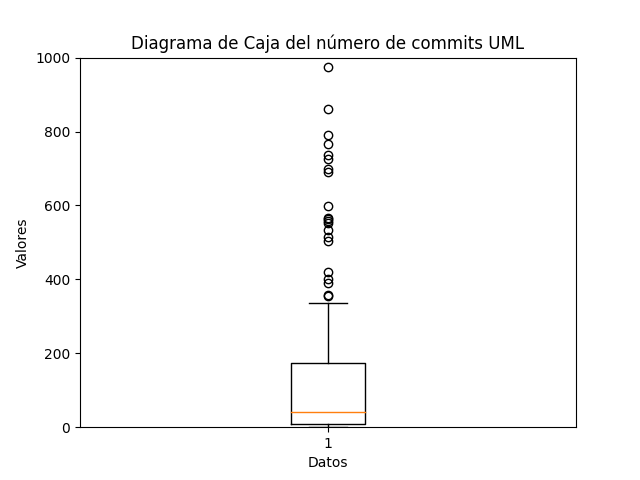
\includegraphics[width=9cm, keepaspectratio]{img/Figure_commitsUML.png}
    \caption{Diagrama de caja del número de commits total por repositorio con diagrama UML. }\label{fig:Figure_commitsUML}
  \end{subfigure}
  \hfill
    \begin{subfigure}{0.45\linewidth}
      \centering
      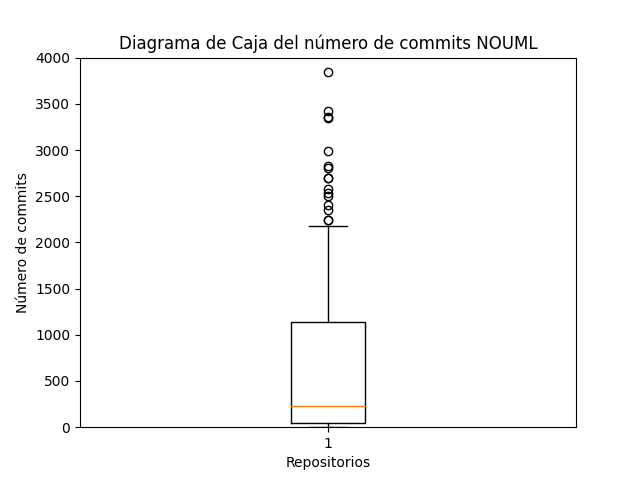
\includegraphics[width=9cm, keepaspectratio]{img/Figure_commitsNOUML.png}
      \caption{Diagrama de caja del número de commits total por repositorio sin diagrama UML.}\label{fig:Figure_commitsNOUML}
  \end{subfigure}
\end{figure}

\section{Conclusiones de los resultados del análisis}
\label{sec:conclusiones de los resultados del análisis}

En este Trabajo de Fin de Grado se ha llevado a cabo un análisis de 400 repositorios de GitHub, para obtener qué patrones tienen los repositorios que poseen modelos UML y qué patrones tienen los repositorios que no utilizan este tipo de modelos.
A través de la recopilación y el análisis de los datos se logró obtener información sobre los repositorios que contienen diagramas UML y los que no contienen diagramas UML.

Después de observar detenidamente los resultados obtenidos en el análisis, podemos decir que algunas de las pautas de nuestra hipótesis no se han cumplido.


A continuación, se van a mencionar los hallazgos que revelan patrones que nos permiten sacar conclusiones significativas sobre los repositorios.

En cuanto al lenguaje de programación que predomina en repositorios con y sin diagramas UML, los resultados muestran que Java es el lenguaje de programación más utilizado en ambos tipos de repositorios, lo cual respalda la hipótesis planteada.
Este hallazgo indica que existe una preferencia generalizada por Java en la comunidad de desarrollo de los repositorios, independientemente de si contienen diagramas UML o no.
Otro dato significativo es que los repositorios con diagramas UML tienen una tendencia clara tener licencias, en comparación con los repositorios que no contienen diagramas UML.


Si nos fijamos en los propietarios de los repositorios, se evidencia un patrón claro de que los repositorios con y sin diagramas UML están predominantemente asociados a propietarios que son usuarios individuales.
Esta tendencia no se cumple, invalidando la hipótesis inicial según la cual se esperaba que los repositorios con diagramas UML estuvieran asociados a propietarios que fueran organizaciones.


Los resultados obtenidos también revelan una tendencia clara en cuanto al tamaño de los repositorios que contienen diagramas UML y los que no contienen diagramas UML.
Esta tendencia respalda nuestra hipótesis al obtener como resultado que los repositorios que contienen diagramas UML tienen un tamaño mayor que los repositorios que no contienen diagramas UML.
Otro hallazgo significativo es que los repositorios con diagramas UML tienen una tendencia clara a tener un menor número de stars y fork que los repositorios que no contienen diagramas UML.
Estos nos revela que son repositorios que tienen un menor apoyo por parte de la comunidad de software que los repositorios que no contienen diagramas UML.


Por último, cabe mencionar que los resultados obtenidos muestran que los repositorios que contienen diagramas UML tienen un número menor de colaboradores y un número menor de commits que los repositorios que no contienen diagramas UML.
Estos resultados no coinciden con nuestra hipótesis inicial, ya que esperábamos que los repositorios que contienen diagramas UML tuvieran un número mayor de colaboradores y un número mayor de commits que los repositorios que no contienen diagramas UML.
Por tanto, podemos concluimos que los repositorios que contienen diagramas UML tienen un mayor tamaño, pero tienen menos colaboradores y menos commits que los repositorios que no contienen diagramas UML.

Con todos estos hallazgos podemos hacer una descripción general de las características que tienen los repositorios que contienen diagramas UML y los que no contienen diagramas UML.

%%%%%%%%%%%%%%%%%%%%%%%%%%%%%%%%%%%%%%%%%%%%%%%%%%%%%%%%%%%%%%%%%%%%%%%%%%%%%%%%
%%%%%%%%%%%%%%%%%%%%%%%%%%%%%%%%%%%%%%%%%%%%%%%%%%%%%%%%%%%%%%%%%%%%%%%%%%%%%%%%
% CONCLUSIONES %
%%%%%%%%%%%%%%%%%%%%%%%%%%%%%%%%%%%%%%%%%%%%%%%%%%%%%%%%%%%%%%%%%%%%%%%%%%%%%%%%

\cleardoublepage
\chapter{Conclusiones}
\label{chap:conclusiones}

Por último, presentamos las conclusiones obtenidas tras realizar este Trabajo de Fin de Grado, en el cual se ha realizado un exhaustivo análisis de 400 repositorios, almacenados en la API de GitHub, para obtener qué patrones tienen los repositorios que poseen modelos UML y cuáles los repositorios que no tienen este tipo de modelos. 
También se realizará una retrospección acerca de los conocimientos adquiridos a lo largo de este proyecto y a lo largo de mi formación académica que han sido esenciales para el desarrollo del mismo.
Además, para concluir, se mencionarán futuras mejoras para perfeccionar o incrementar la funcionalidad de los programas realizados para conseguir llevar a cabo un análisis más exhaustivo con el que se podrían ampliar y enriquecer los resultados obtenidos.


\section{Consecución de objetivos}
\label{sec:consecucion-objetivos}

Basándonos en los resultados obtenidos y el análisis realizado, se puede concluir que se ha logrado cumplir satisfactoriamente el objetivo general de este Trabajo de Fin de Grado.
Durante la realización de este proyecto nos hemos ido enfrentando a los desafíos de cada uno de los objetivos específicos que se muestran en el capítulo ~\ref{chap:objetivos}.
Dentro de los objetivos planteados, se ha logrado realizar un aprendizaje de la herramienta Perceval, que nos ha permitido recopilar los datos de los repositorios que se han seleccionado en documentos estructurados JSON, para realizar el análisis de este proyecto. 
También se ha conseguido desarrollar una serie de programas para extraer y almacenar los datos que nos resultaron relevantes para el análisis de nuestro estudio.
Y por último, se ha llevado a cabo con éxito el análisis con el cual se observan las diferencias y similitudes de los repositorios que tienen archivos UML y los que no.
Por tanto, se han completado todos los objetivos propuestos a pesar de las dificultades encontradas.


Con este estudio se pretende aportar una comprensión más profunda sobre las tendencias que siguen los repositorios de GitHub con diagramas UML frente a los que no los usan.


\section{Aplicación de lo aprendido}
\label{sec:aplicacion}

La aplicación de los conocimientos y habilidades adquiridos en mi formación académica en el Grado en Ingeniería en Sistemas Audiovisuales y Multimedia ha sido esencial para la elaboración de este Trabajo de Fin de Grado.
A continuación, se mencionan los aprendizajes que me permitieron realizar la extracción, tratamiento y clasificación de datos para obtener como resultado el análisis de este proyecto. 

\begin{enumerate}
  \item Informática I: Me sirvió fundamentalmente par adquirir las bases de programación.
  \item Informática II: Aparte de reforzar las bases de programación adquiridas, obtuve una formación en otras herramientas comúnmente usadas para programar y, además, mejoré la estructuración de código y lógica necesarias en programación.
  \item Protocolos para la Transmisión de Audio y Vídeo de Internet: En esta materia aprendí los conocimientos del lenguaje de programación Python, además de cómo se estructura y para qué se usa la estructura de datos JSON.
  \item Estadística para Sistema Audiovisuales: La adquisición de conceptos básicos de probabilidad y estadística me ha sido de ayuda en el proceso de análisis de datos de este proyecto. 
\end{enumerate}


\section{Lecciones aprendidas}
\label{sec:lecciones_aprendidas}

Durante la realización de este Trabajo de Fin de Grado, he adquirido diversos conocimientos sobre las herramientas usadas para realizar un análisis de datos. 
A continuación, se presentan algunos de los aprendizajes más significativos que he adquirido:

\begin{enumerate}
  \item  Al inicio de este proyecto lo primero que aprendí fue cómo funciona la herramienta de Perceval. Gracias a ella he podido obtener los datos necesarios para realizar el análisis de este proyecto, que era el objetivo final del mismo. 
  \item  Este proyecto, además, me ha ayudado a entender mejor los tipos de repositorios que se encuentran en GitHub; ya que, analizando las características de estos repositorios se puede sacar mucha información de sus propietarios para ver las características que los definen, tales como si usan licencia, si son usuarios individuales o forman parte de una organización, etc.
  \item  He ampliado mis conocimientos sobre la estructura JSON. Esto me ha servido para comprender porque es comúnmente utilizada para el tratamiento e intercambio de datos, la razón no es otra que su sintaxis sencilla, su formato ligero y su flexibilidad en la estrutura de datos. Además, como he trabajado con archivos JSON durante la realización del proyecto, he mejorado la forma en la que tratar dichos archivos a la hora de extraer y guardar datos en dicha estructura.  
  \item  También, he mejorado mis conocimientos de Python al emplear este lenguaje de programación en el desarrollo de los ficheros que se han usado para el tratamiento de los datos de los archivos JSON obtenidos con Perceval.    
  \item  Utilizar MongoDB ha sido otro de los aprendizajes durante este proyecto; puesto que, no tenía apenas conocimientos de bases de datos y nunca las había utilizado. Asimismo, en este proyecto, he aprendido a usar MongoDB con Python empleando el módulo ``pymongo'' con el que te puedes conectar a MongoDB y trabajar con las bases de datos.
  \item  Aprender a usar el módulo ``subprocess'' ha sido muy útil; puesto que con este módulo he creado un fichero, que introduce todos los documentos JSON en MongoDB, de modo automático al ejecutarlo y esto ha sido de gran utilidad para la realización del trabajo.
  \item  Realizar este proyecto con LaTeX ha sido otra de las lecciones que he adquirido. El aprendizaje de Latex no ha sido muy costoso y gracias a él he podido tener la memoria del Trabajo de Fin de Grado bien estructurada y organizada.
\end{enumerate}


Entre las lecciones aprendidas destacaría también la adquisición o mejora de algunas destrezas necesarias para elaborar un proyecto de estas características:
\begin{enumerate}
  \item  La primera es que este proyecto me ha servido para saber determinar y acotar el objeto de investigación de un proyecto como éste y los pasos a seguir en su desarrollo.
  \item  La planificación y la capacidad para establecer plazos realistas sobre las diferentes etapas del proyecto ha sido otra destreza que he mejorado durante la realización de este Trabajo de Fin de Grado.
  \item  Otra de las destrezas que he desarrollado es a saber elegir y seleccionar, entre la gran cantidad de información que existe, que información es relevante y cual no, puesto que no aporta nada significativo al objeto de investigación.
  \item  También he adquirido la aptitud para resolver y analizar los problemas que pueden surgir en un proyecto de este tipo y buscar posibles soluciones y alternativas.  
  \item  Y, por último, el esfuerzo de síntesis a la hora de redactar el proyecto y que este resulte claro para aquellos que lo lean y quieran realizar o ampliar dicho estudio. 
\end{enumerate}

\section{Trabajos futuros}
\label{sec:trabajos_futuros}


En relación a los trabajos futuros, se pueden realizar varias mejoras para llevar a cabo futuros análisis más exhaustivos de los repositorios de GitHub que contengan diagramas UML y así poder obtener un conocimiento mayor sobre las características que presentan los repositorios con diagramas UML que pueda ser útil para la comunidad de ingeniería de software. 
A continuación, se mencionarán algunas de las mejoras o nuevas funcionalidades de la herramienta que proponemos:

\begin{itemize}
  \item  Una posible mejora podría ser la forma en la que nuestra herramienta detecta si hay diagramas UML o no.
  \item  Para mejorar este estudio se debería realizar un análisis de un mayor número de repositorios.
  \item  También podría ser interesante implementar en el programa la funcionalidad para saber el tipo de archivos que se han usado para almacenar estos diagramas UML.
\end{itemize}



%%%%%%%%%%%%%%%%%%%%%%%%%%%%%%%%%%%%%%%%%%%%%%%%%%%%%%%%%%%%%%%%%%%%%%%%%%%%%%%%
%%%%%%%%%%%%%%%%%%%%%%%%%%%%%%%%%%%%%%%%%%%%%%%%%%%%%%%%%%%%%%%%%%%%%%%%%%%%%%%%
% APÉNDICE(S) %
%%%%%%%%%%%%%%%%%%%%%%%%%%%%%%%%%%%%%%%%%%%%%%%%%%%%%%%%%%%%%%%%%%%%%%%%%%%%%%%%

% \cleardoublepage
% \appendix
% \chapter{Manual de usuario}
% \label{app:manual}

% Esto es un apéndice.
% Si has creado una aplicación, siempre viene bien tener un manual de usuario.
% Pues ponlo aquí.

%%%%%%%%%%%%%%%%%%%%%%%%%%%%%%%%%%%%%%%%%%%%%%%%%%%%%%%%%%%%%%%%%%%%%%%%%%%%%%%%
%%%%%%%%%%%%%%%%%%%%%%%%%%%%%%%%%%%%%%%%%%%%%%%%%%%%%%%%%%%%%%%%%%%%%%%%%%%%%%%%
% BIBLIOGRAFIA %
%%%%%%%%%%%%%%%%%%%%%%%%%%%%%%%%%%%%%%%%%%%%%%%%%%%%%%%%%%%%%%%%%%%%%%%%%%%%%%%%

\cleardoublepage
% \chapter*{Bibliografía}
% \label{app:bibliografía}

% Las siguientes dos instrucciones es todo lo que necesitas
% para incluir las citas en la memoria
\bibliographystyle{abbrv}
\bibliography{memoriaTFG}  % memoria.bib es el nombre del fichero que contiene


% las referencias bibliográficas. Abre ese fichero y mira el formato que tiene,
% que se conoce como BibTeX. Hay muchos sitios que exportan referencias en
% formato BibTeX. Prueba a buscar en http://scholar.google.com por referencias
% y verás que lo puedes hacer de manera sencilla.
% Más información: 
% http://texblog.org/2014/04/22/using-google-scholar-to-download-bibtex-citations/

\end{document}
